\documentclass{article}[12pt]

\usepackage{graphicx}

\begin{document}

\title	{A High Temperature Superconducting\\ Microwave Filter \\ for the Narrabri Radio Telescope}
\author	{Ben Lippmeier}
\date	{February 2001}

\maketitle

\begin{abstract}
We design the design and construction of a High Temperature Superconducting (HTS) microwave filter to block the interference being suffered by the Narrabri Compact Array radio observatory between 2300 and 2400 MHz. After a successful copper prototype, the HTS filter was fabricated and tested. The filter response had the correct shape though the center frequency was 35MHz too high due to simulation and fabrication tolerances. Future work will be to produce a filter which has a center frequency around 50MHz lower than the current design, and trim the resonators down until it is at the correct frequency.
\end{abstract}

%!TEX root = ../Main.tex
\section{Project Overview}
The compact array operates on four main observing bands:

\begin{itemize}
\item	1250-1760 MHz (20cm - L-Band)
\item	2200-2500 MHz (13cm - S-Band)
\item	4400-6860 MHz (6cm  - C-Band)
\item	8000-9200 MHz (3cm  - X-Band)
\end{itemize}

All four of these bands are suffering increasing levels of interference from terrestrial and orbital sources due to the proliferation of radio communication systems and RFI emitting equipment. Specific sources of interference include microwave ovens, cell phones, computer equipment, navigation satellites (GPS, GLONASS), microwave point to point links and the microwave multipoint distribution systems (MDS) used for pay-TV. These problems are compounded by the fact that the signal levels of interest to astronomers are many orders of magnitude less than even the higher harmonics of terrestrial transmissions.

In 1996, a MDS network servicing Narrabri and the surrounding region began operating between 2300 and 2400MHz, which falls in the middle of the 13cm band. This service is a broadcast system transmitting from a tower located about 55 km away on nearby mount Kaputar. Although the service is transmitting within their allocated band, the ATNF astronomers wish to observe close the 2300MHz band edge, as this frequency is close to the lower limit of the Tidbinbilla 70m S-band maser amplifier which is used for Very Long Baseline Interferometry (VLBI) observations. Unfortunately, the existing telescope receivers have limited preselect-filtering, so by the time the MDS signal has been amplified and down converted, its bottom edge is still of sufficient magnitude to saturate the samplers and noise temperature measurement system.

My project was to produce a preselect filter to allow observations right next to the lower edge of the MDS band. After corresponding with the staff at Narrabri, it was decided that a clear 64MHz pass band centered on 2260 (range from 2228 to 2292 MHz) would be a vast improvement over their current arrangement. The target was 20dB attenuation at 2300MHz and as much possible over the MDS band.
%!TEX root = ../Main.tex

% ------------------------------------------------------------------
\section{Design Process}
Hong and Lancaster~\cite{hong:microstrip} describe a class of filters that would provide the required response if fabricated in high temperature superconducting (HTS) material. As any pre-select filter would need to be installed along with the low noise amplifiers, and cooled to 20K, using superconducting material would make good use of the existing equipment. However, as we did not have the ability to fabricate a HTS device in-house, we decided to first produce a copper prototype to test the theory.

% ------------------------------------------------------------------
\subsection{Quazi-elliptic resonant filters}
The filter design described in~\cite{hong:microstrip} consists of a set of coupled planar resonators arranged to give a quazi-elliptic response. A quazi-elliptic response is similar to a Chebyshev response, except that a pair of transmission zeros have been moved from infinity down next to the passband. This provides the steep skirts in the filter response, as shown in Figure~\ref{figure:quazi-elliptic-8-pole-ideal}.

\begin{figure}[ht]
\begin{center}
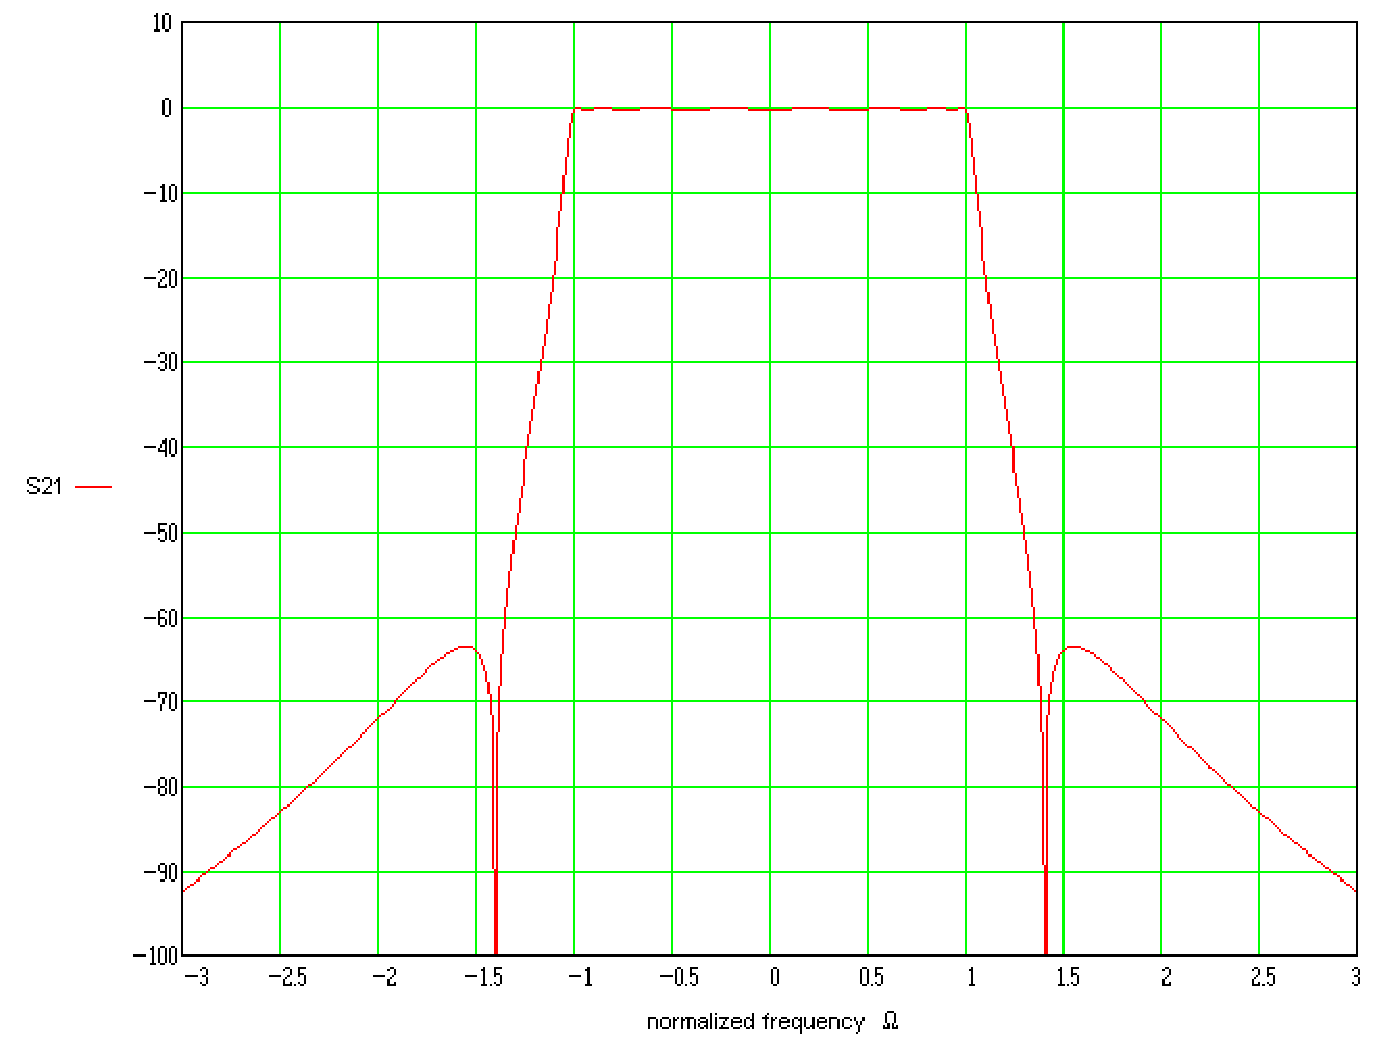
\includegraphics[scale=0.5]{fig/quazi-elliptic-8-pole-ideal.pdf}
\end{center}
\caption{8-pole quazi-elliptic filter ideal response}
\label{figure:quazi-elliptic-8-pole-ideal}

\end{figure}
The finite frequency zeros are obtained by having two separate signal paths in the filter. Figure \ref{figure:signal-paths} also shows a possible layout that includes two signal paths, the primary one through resonators 1-2-3-4-5-6-7-8, and a secondary one through 1-2-3-6-7-8. When the signals transmitted through both of these paths are $180^\circ$ out of phase at the output port, they cancel and provide the transmission zeros in the filter response.

\begin{figure}
\begin{center}
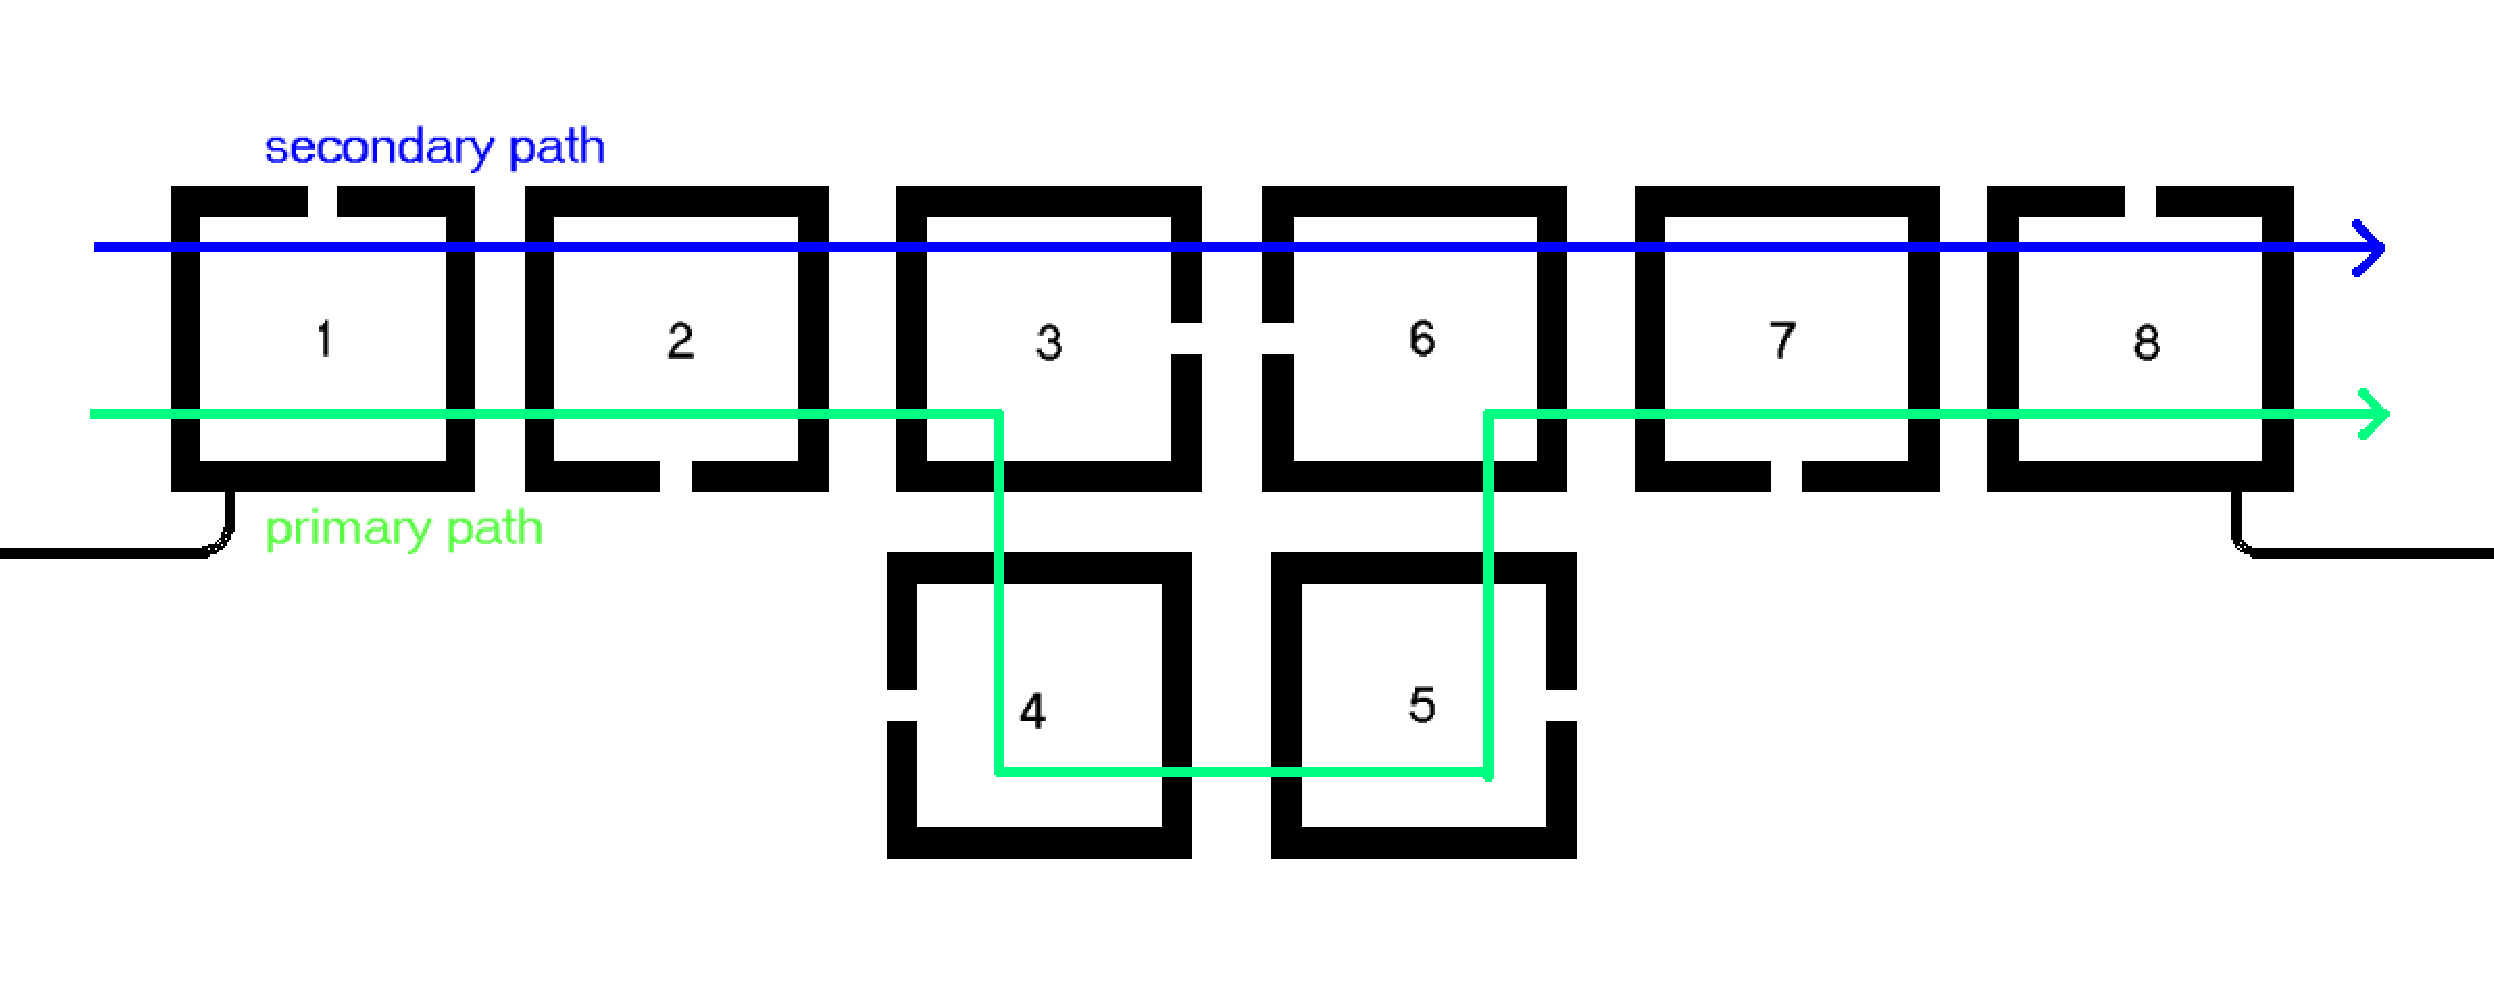
\includegraphics[scale=0.3]{fig/quazi-elliptic-8-pole-layout-path.pdf}
\end{center}
\caption{Primary and secondary signal paths}
\label{figure:signal-paths}
\end{figure}


% ------------------------------------------------------------------
\subsection{Choosing Design Parameters}
The desired filter has a passband of 2228-2292MHz with 20dB attenuation at 2300MHz. We used the filter equations of~\cite{hong:microstrip} to determine the parameters needed to meet this specification. The key parameters are the order, which is identical to the number of resonators in the circuit, and the filter parameter $\Omega_a$, which controls how close the transmission zeros are to the passband. Figure \ref{figure:filter-variation} shows the effect of changing these two parameters. Note that having zeros close to the passband provides a steeper skirt, but the two large ripples in the stop-band rise up and reduce the isolation of the filter.

We chose an 8th order filter to provide the required selectivity, while widening the design bandwidth to 68Mhz to allow some slack in the center frequency of the filter. The value of $\Omega_a$ was set to 1.4 as it provided a tradeoff between selectivity and isolation. An ideal filter with these parameters would provide 30dB attenuation at 2300MHz, which allows slack to compensate for fabrication tolerances and rounding of the response due to electrical losses.

\begin{figure}[ht]
\begin{center}
\hspace{-8em}
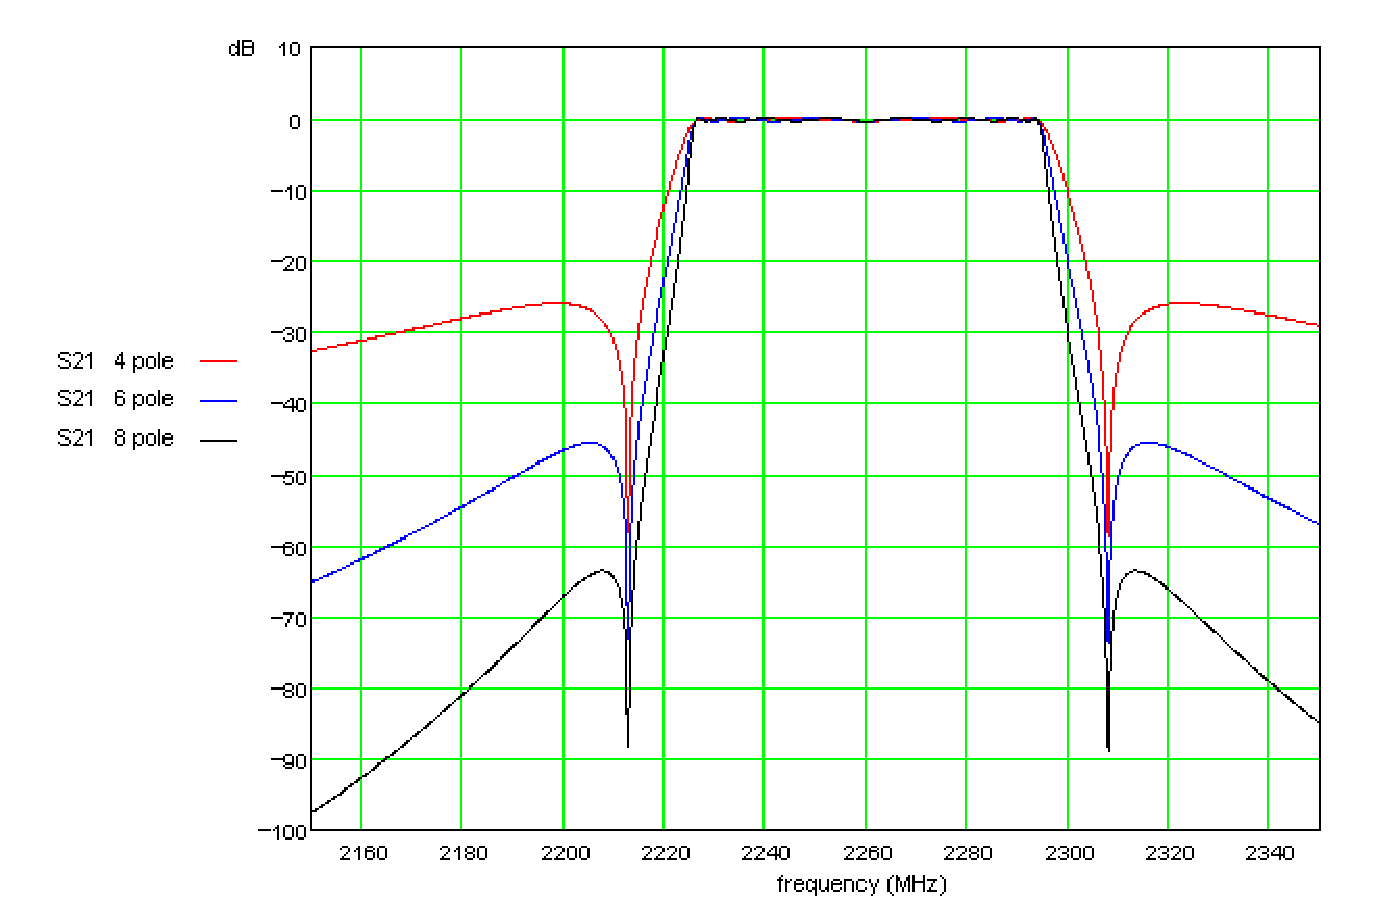
\includegraphics[scale=0.6]{fig/design-vary-order.pdf}

\hspace{-8em}
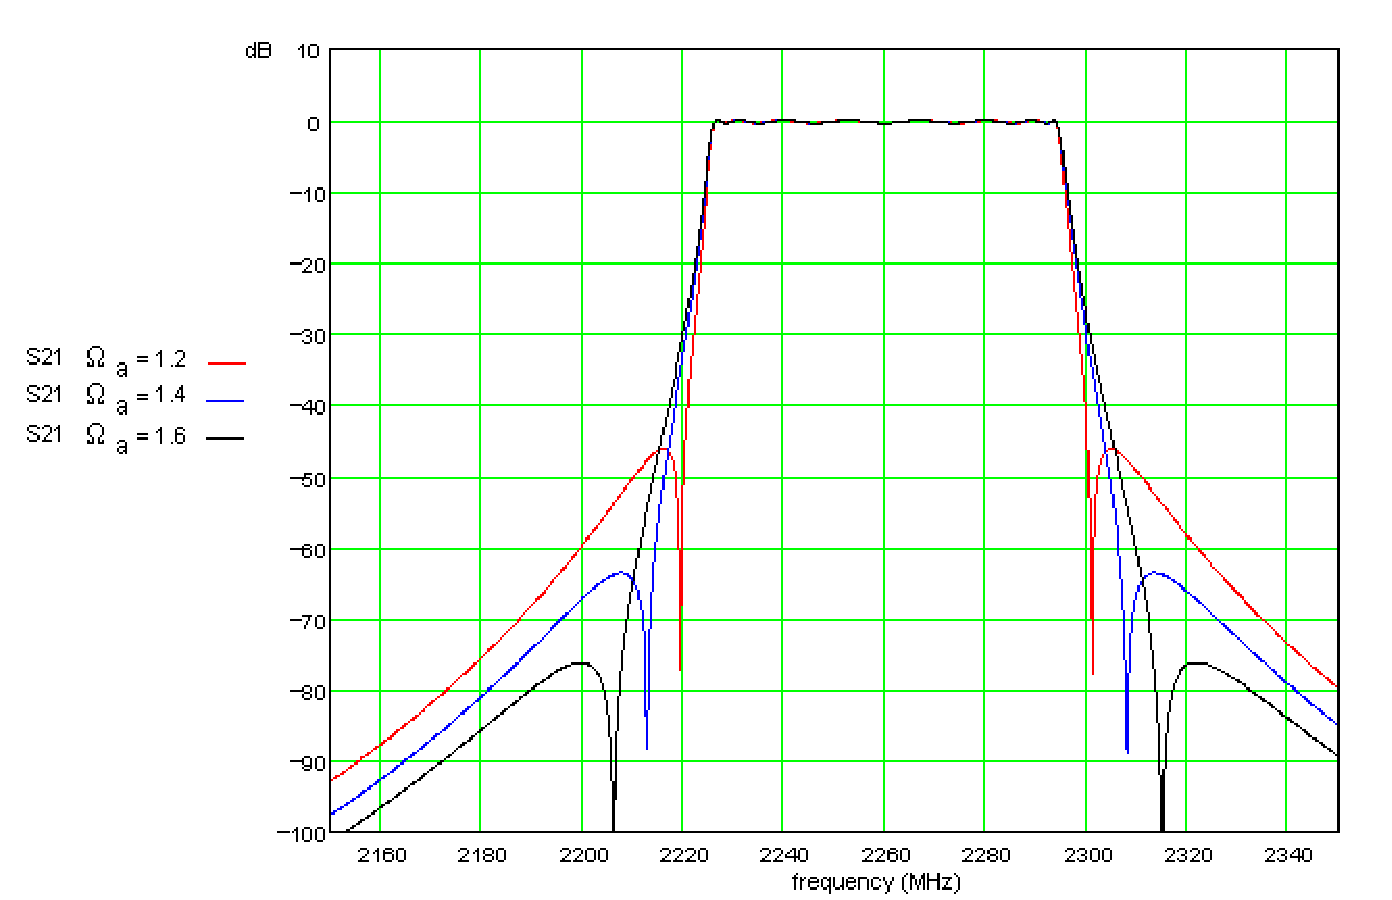
\includegraphics[scale=0.6]{fig/design-vary-omega.pdf}
\end{center}

\caption{Variations in filter response due to changing its order and $\Omega_a$}
\label{figure:filter-variation}
\end{figure}


% ------------------------------------------------------------------
\subsection{Detailed Design}
After the main parameters had been chosen, the detailed design consisted of taking one of the standard layouts and setting the length of the resonators to resonate at the desired center frequency. Next, we adjust the coupling between each pair of adjacent resonators to provide the desired quazi-elliptic response. 

In Figure~\ref{figure:signal-paths} note that there are four types of resonator couplings, where the type of coupling depends on how the resonators are arranged with respect to each other. The couplings are named electric, magnetic, mixed and hybrid, and are shown in Figure \ref{figure:design-couplings}

\begin{figure}[ht]
\begin{center}
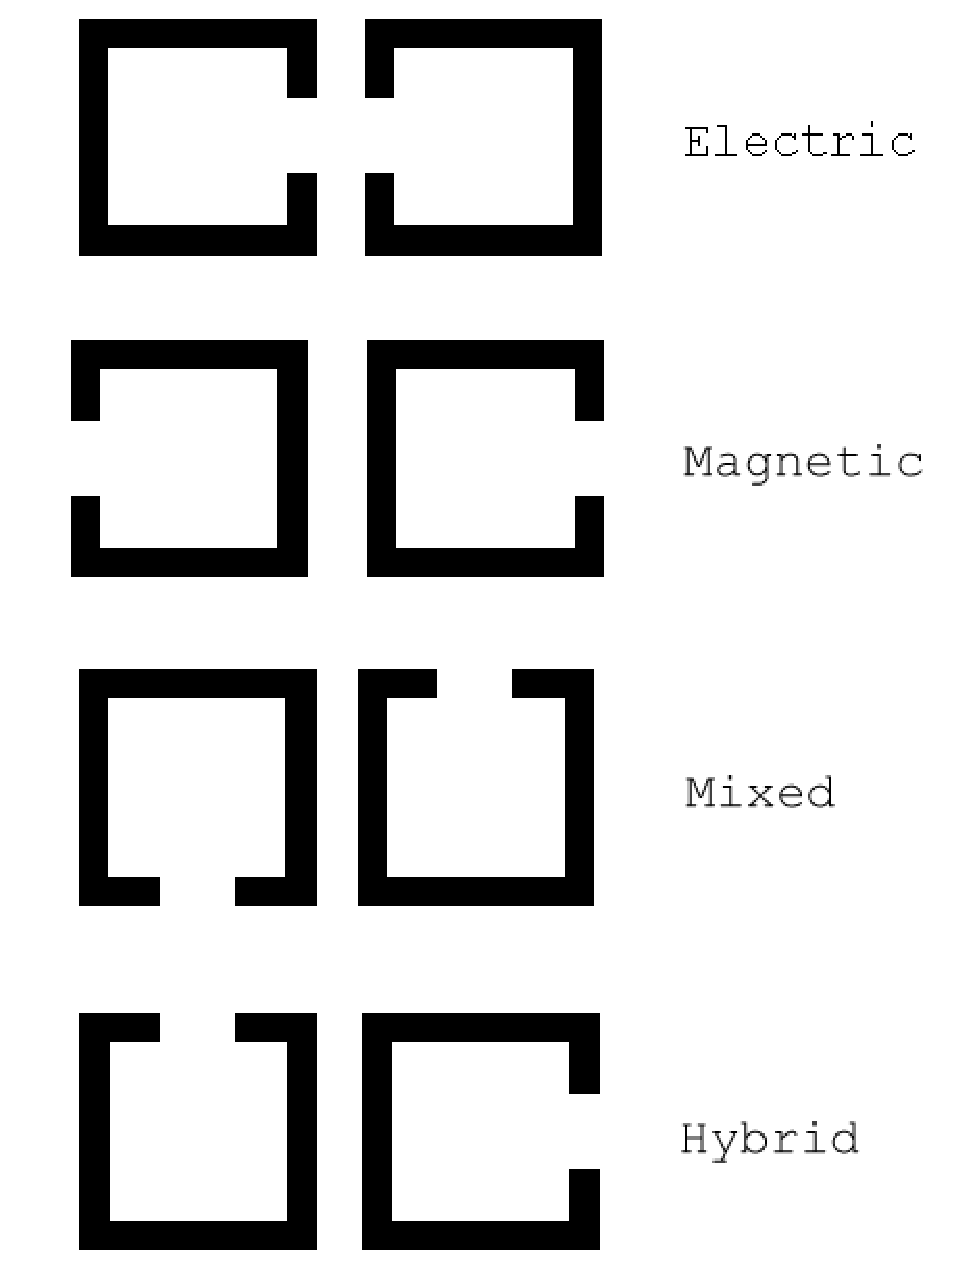
\includegraphics[scale=0.3]{fig/design-couplings.pdf}
\end{center}
\caption{Possible resonator couplings}
\label{figure:design-couplings}
\end{figure}

The coupling names ``electric'' and ``magnetic'' refer to the field that provides the coupling, and ``mixed'' and ``hybrid'' make use of both fields. An important point is that electric coupling provides a phase inversion with respect to the other types, and this is used to produce the transmission zeros in the filter response.

Once the filter layout has been chosen, the remaining design variables are the length of the resonators, and the distance between them. The resonator length sets the center frequency, and the coupling coefficents set the $\Omega_a$ parameter.


% ------------------------------------------------------------------
\subsubsection{Length of resonators}
The length of each resonator corresponds to half the wavelength at the filter's center frequency. For the copper prototype we planned to use RT Copper/Duroid 6010.5 as the substrate, which has E=10.5 and h=0.635. We used the Winline program produced by Eagleware to determine the required resonator length (about 28mm). We also used this program to calculate the width of a 50 Ohm feed line to be 0.6mm.


% ------------------------------------------------------------------
\subsubsection{Coupling coefficients}
A set of tables which state the required coupling coefficients was provided in \cite{hong:microstrip}, and \cite{hong:couplings} explains how to determine the resonator separation needed to achieve these coefficients.

Although two identical resonators have the same center frequency, when they are brought close together their fields begin to overlap. This coupled system resonates at seperate resonant frequencies, where the difference between the two frequencies increases with coupling coefficient. The coupling coefficient is determined by the proximity between the two resonators, so as they are brought closer the coefficient increases, and difference between the two resonant frequencies also increases. Figure \ref{figure:design-resonant-frequeny-splitting} shows how the filter response of two 28mm resonators varies as the separation is reduced.

\begin{figure}
\hspace{-4em}
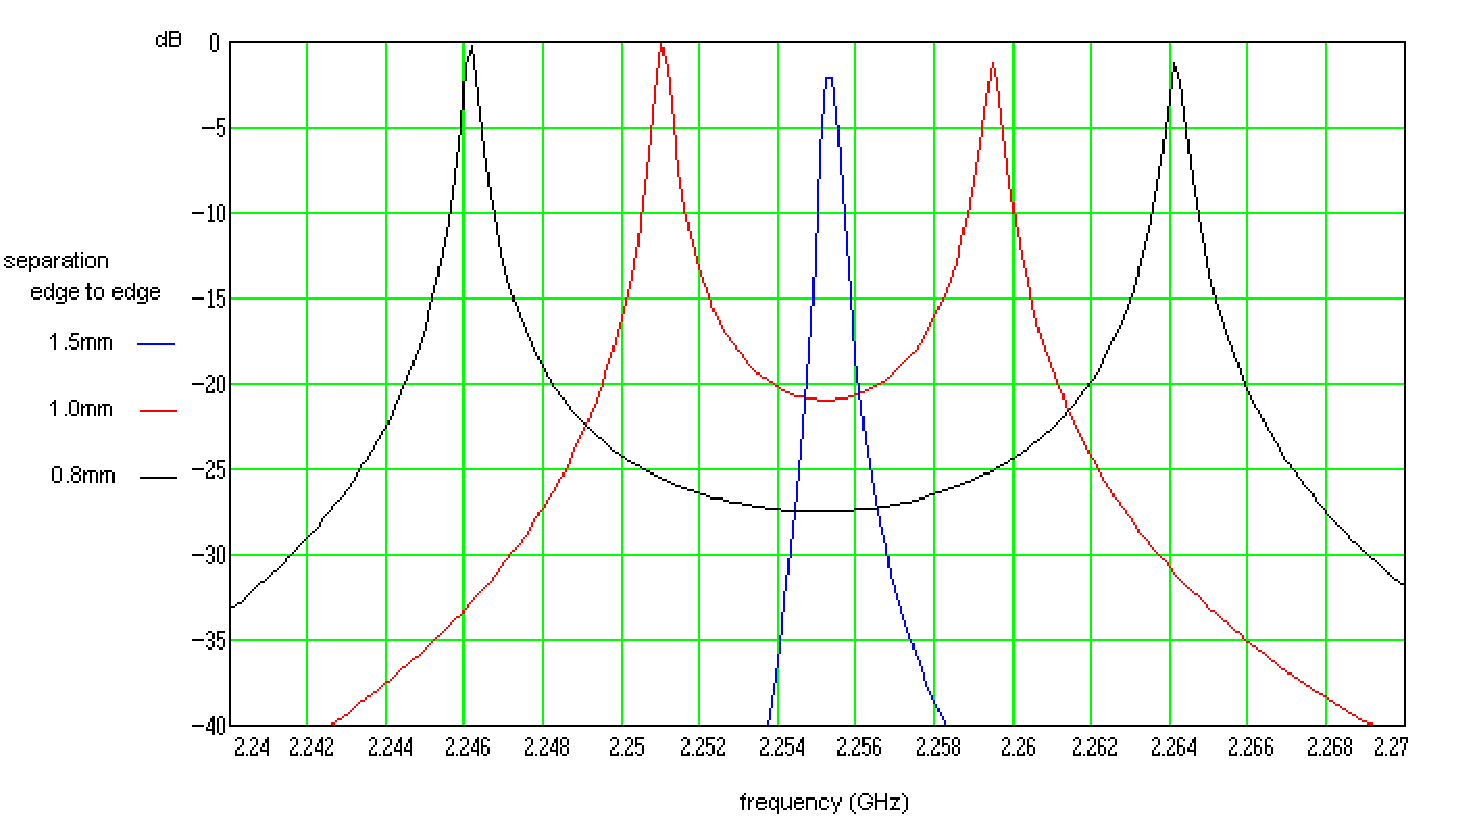
\includegraphics[scale=0.6]{fig/design-resonant-frequency-splitting.pdf}
\caption{Filter response \emph{vs} distance between coupled resonators}
\label{figure:design-resonant-frequeny-splitting}
\end{figure}

If the two resonant frequencies are $f$ and $g$, then coupling coefficient $M$ can be determined from the following equation:
$$
M = 	\frac	{f^2 - g^2}
		{f^2 + g^2}
$$

We can also control the coupling coefficient by varying the width of the resonator track, whereby reducing the width of the track increases the coupling coefficient. Note that as the resonator tracks have a finite width, there is a degree of uncertainty as to the exact length of the track seen by the resonant wave. Some trial and error is needed to determine the dimensions of the resonator. 

To determine the physical sepration required to achieve each coupling coefficient, we used the Ensemble EM simulation software by Ansoft. The process consisted of making a guess at the separation required, and then simulating a system of two coupled resonators to determine its filter response. We calculated the coupling coefficient via the above equation, and if it wasn't close enough, adjusted the separation and tried again.

Note that as the coupling between each resonator is via fringe fields, a `Full Wave' analysis package such as Ensemble must be used as it simulates the full field pattern around a planar structure. These full wave packages are different from transmission line simulators which simulate circuits via transmission line analysis, tabulated S-parameters and lumped element models for discontinuities such as corners, vias and T-sections.

We found Ensemble's simulation times to be reasonable, taking about 5 minutes to calculate 200 frequency points for two resonator circuit on Pentium II 400MHz /128MB workstation. However, as it has no automatic optimization capability, all circuit modifications had to be done by hand in the provided editor. Often the time involved in changing the circuit was more than the simulation time. Quite a few days of work could have been saved if some form of scripting language was available to set up a circuit such as in Figure~\ref{figure:design-couplings} and then take five or six frequency plots at different separations.


% ------------------------------------------------------------------
\subsubsection{Putting it together}
Once the resonator separations were determined we constructed the entire filter in Ansoft, and calculated its response. 50 Ohm lines were used to get the signal in and out of the filter, and their position along the first and last resonators determines the external Q factor of the circuit.

The first filter layout we tried, shown in Figure~\ref{figure:filter-missing-zero-layout}, had a dissapointing response. As we can see from Figure~\ref{figure:filter-missing-zero-response} the zero to the left of the pass-band is missing, and the one on the right is too high in frequency. After some investigation we decided that although arranging the resonators in this way reduces the physical size of the filter compared with the one in Figure \ref{figure:signal-paths}, it also introduces couplings between non adjacent resonators. Extra couplings such as the ones between resonators 1-3, 2-4, 3-5 and so on were not counted for in the filter design, but when simulated we determined their coefficients to be only one order of magnitude lower than the wanted couplings. Others have reported similar problems~\cite{hong:performance}. 

\begin{figure}[ht]
\begin{center}
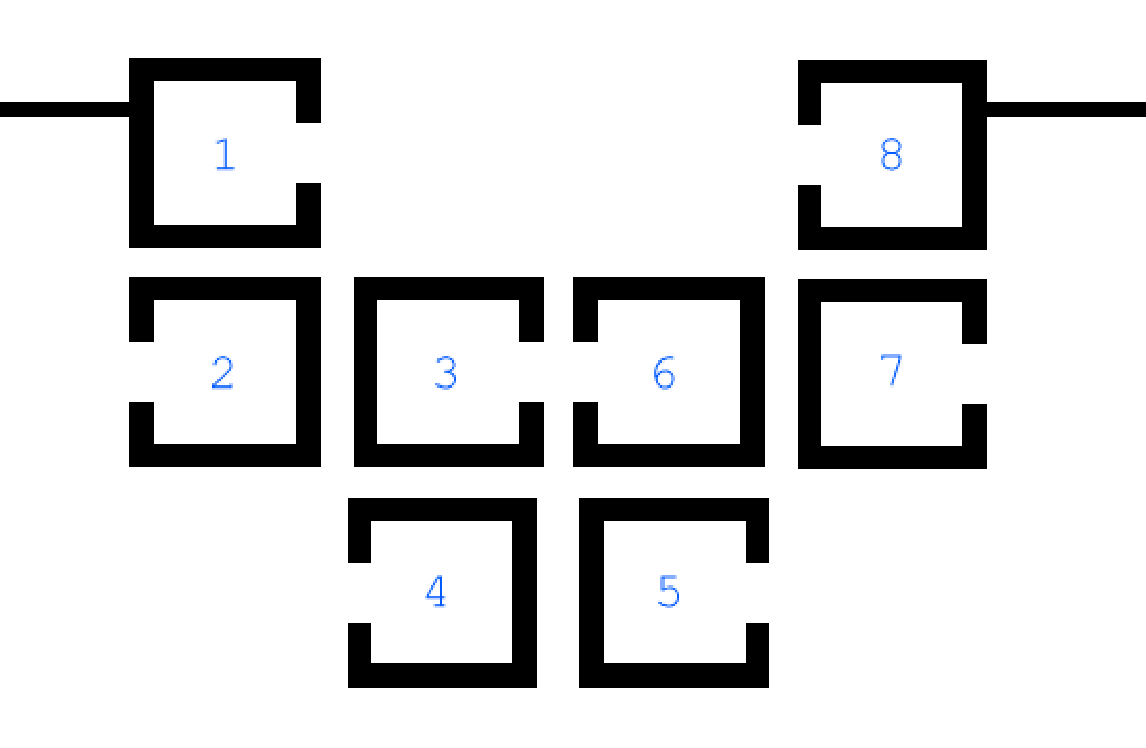
\includegraphics[scale=0.4]{fig/design-bad-8-pole-layout.pdf}
\end{center}
\caption{Filter layout with unwanted couplings}
\label{figure:filter-missing-zero-layout}
\end{figure}

\begin{figure}[ht]
\hspace{-4em}
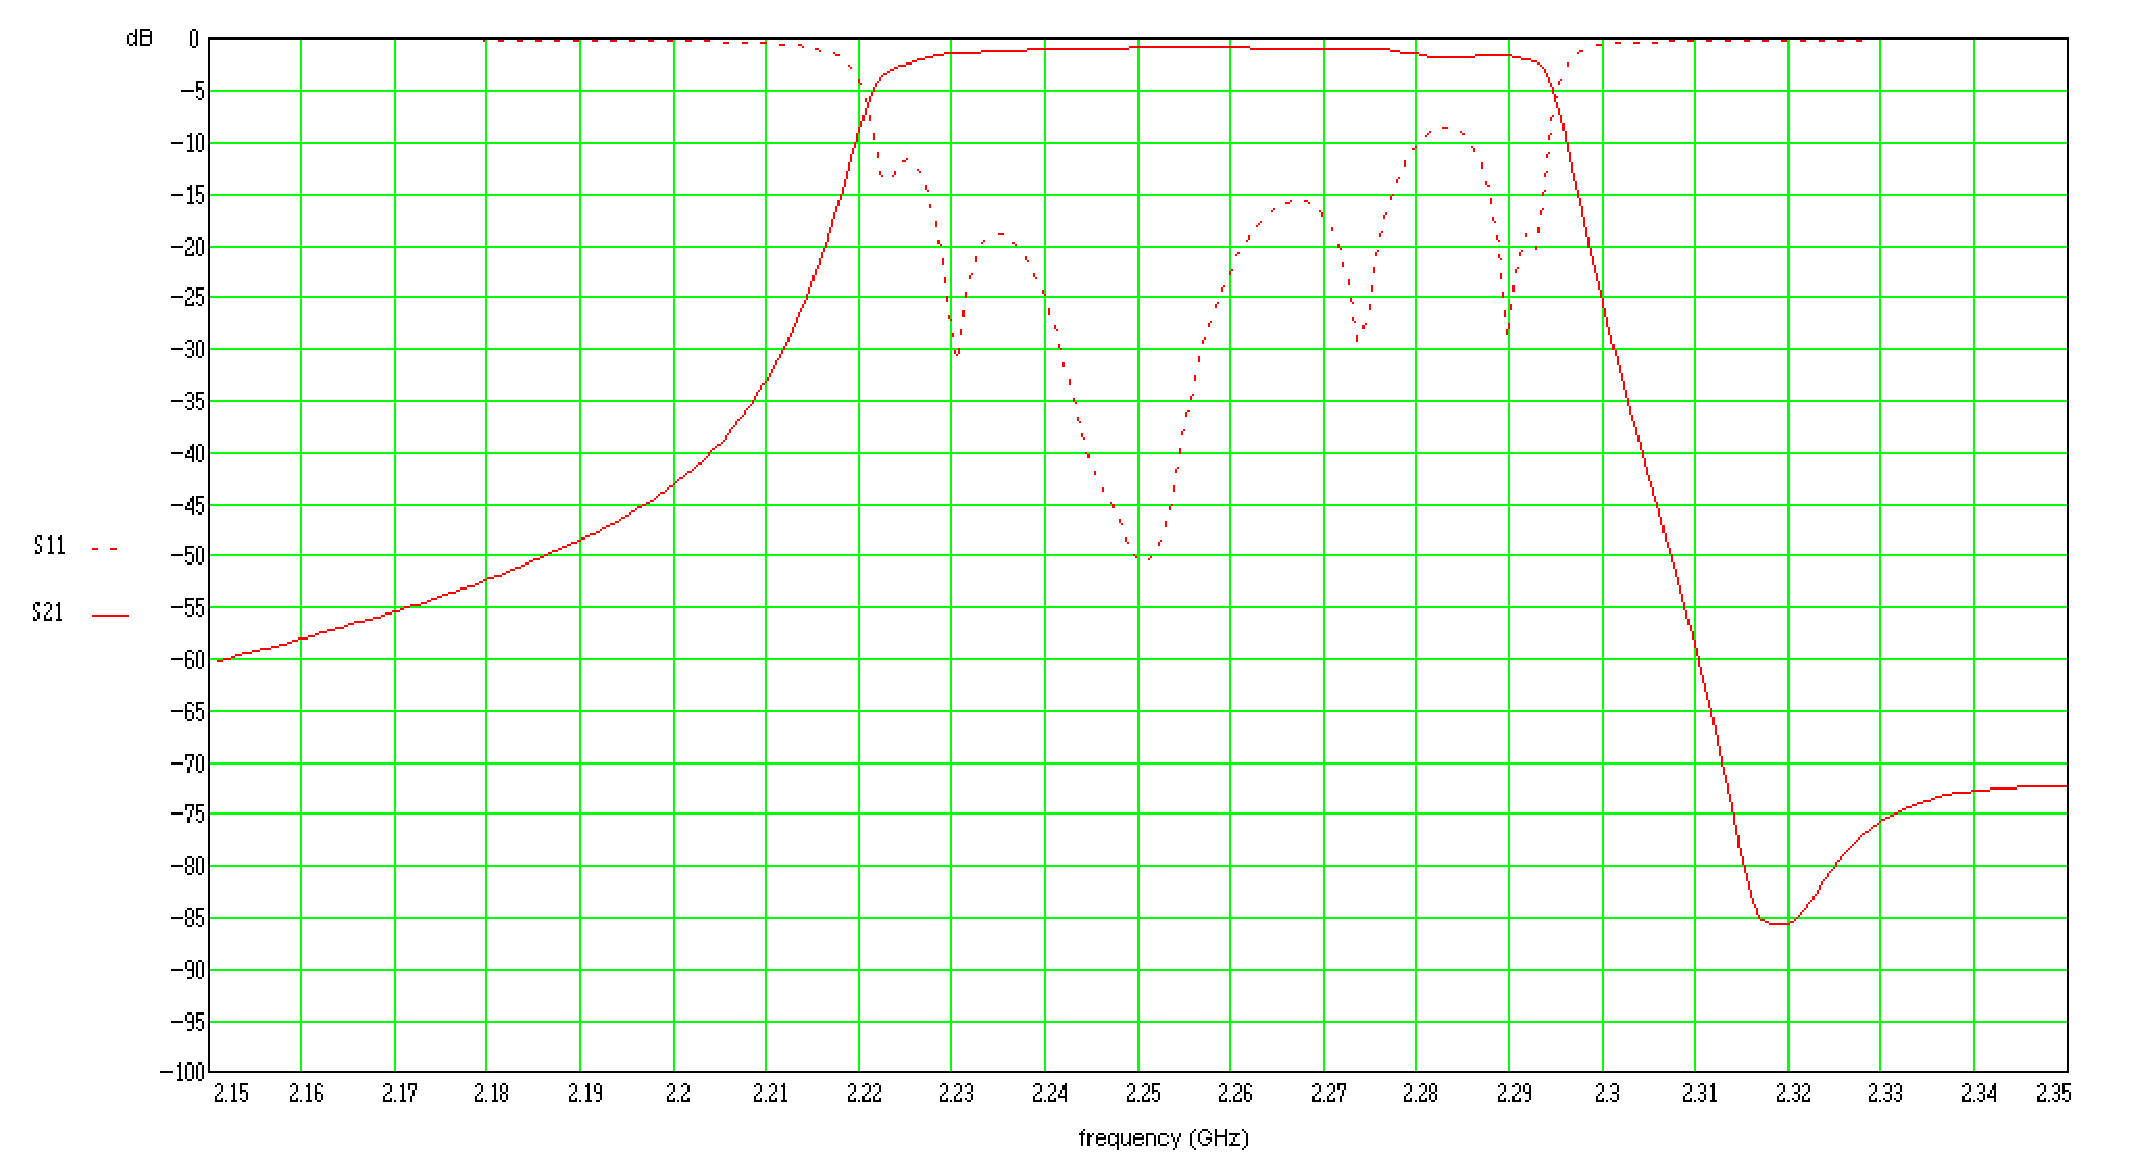
\includegraphics[scale=0.4]{fig/design-bad-8-pole-response.pdf}
\caption{Filter response with missing zero}
\label{figure:filter-missing-zero-response}
\end{figure}

To counter this problem we redesigned the filter to separate resonators 1-3 and 6-8. The final layout is shown in Figure \ref{figure:design-copper-layout} and its simulated response in Figure~\ref{figure:design-copper-response}.


\begin{figure}[ht]
\begin{center}
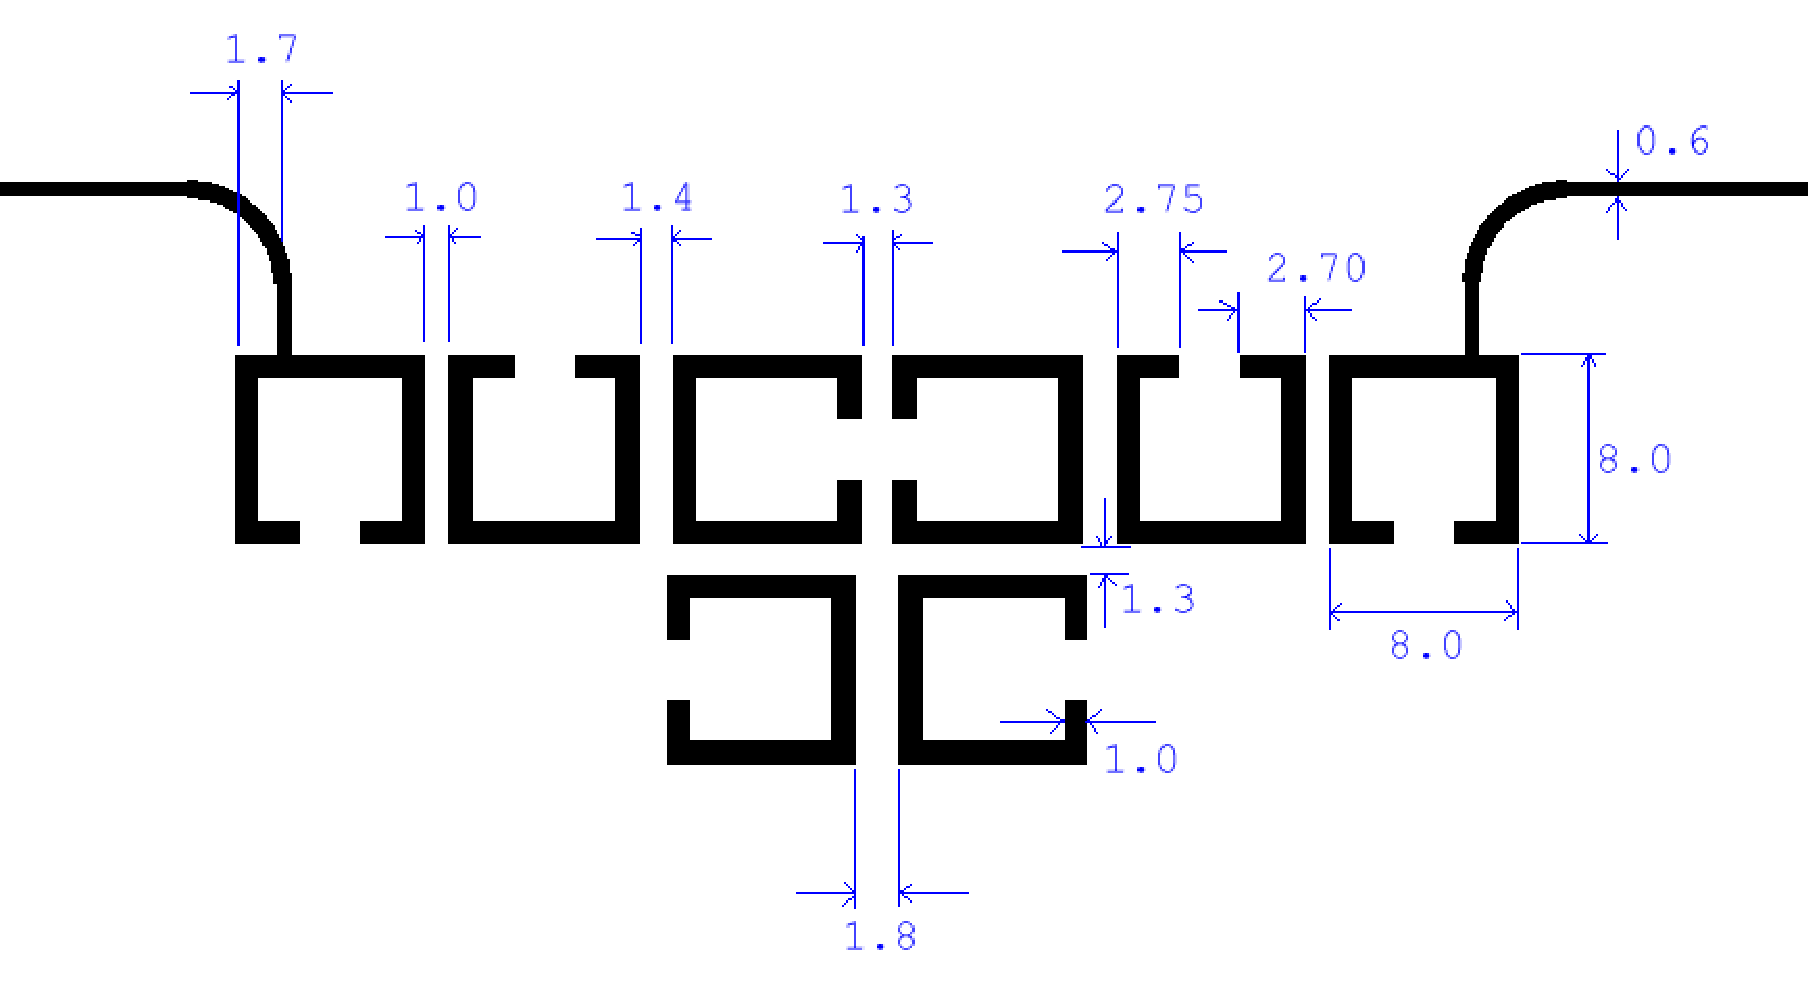
\includegraphics[scale=0.4]{fig/design-copper-layout.pdf}
\end{center}
\caption{ Final layout for copper filter (dimensions in mm)}
\label{figure:design-copper-layout}
\end{figure}

\begin{figure}[ht]
\hspace{-4em}
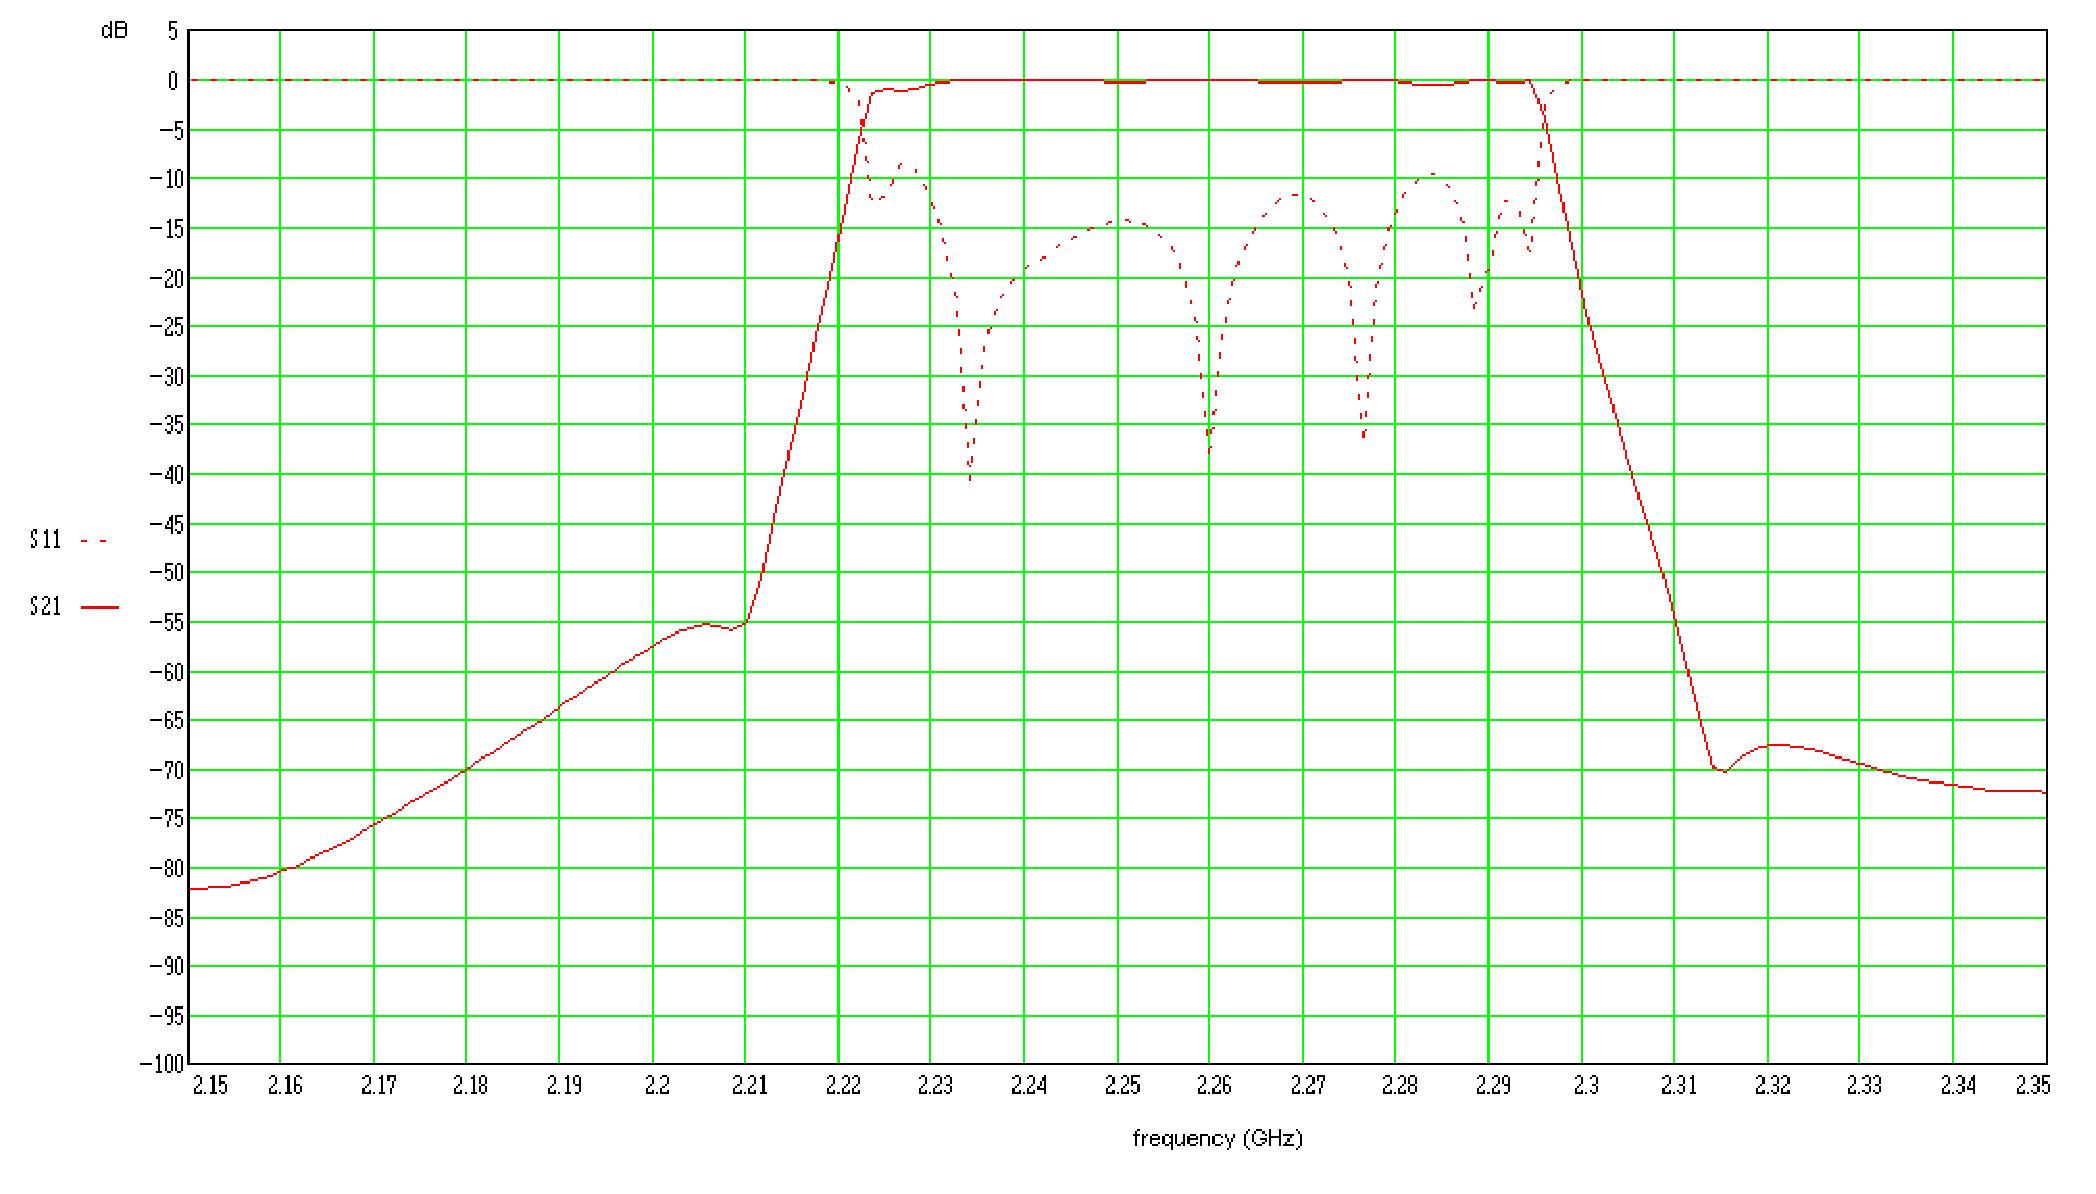
\includegraphics[scale=0.4]{fig/design-copper-simulated.pdf}
\caption{Simulated response of copper filter}
\label{figure:design-copper-response}
\end{figure}


%!TEX root = ../Main.tex
\section{Fabrication of Copper Test Filter}

Once the design was finalised we plotted the circuit in Protel and had photo masks made. We also made masks to verify our method of calculating resonator coupling coefficients. Fabrication consisted of spinning photo resist onto the Duroid board, exposing it with the mask under UV light then etching. The copper filter is shown in Figure \ref{figure:test-copper-open}, and resonator boards are shown in Figure \ref{figure:test-resonator-open}.

\begin{figure}[ht]
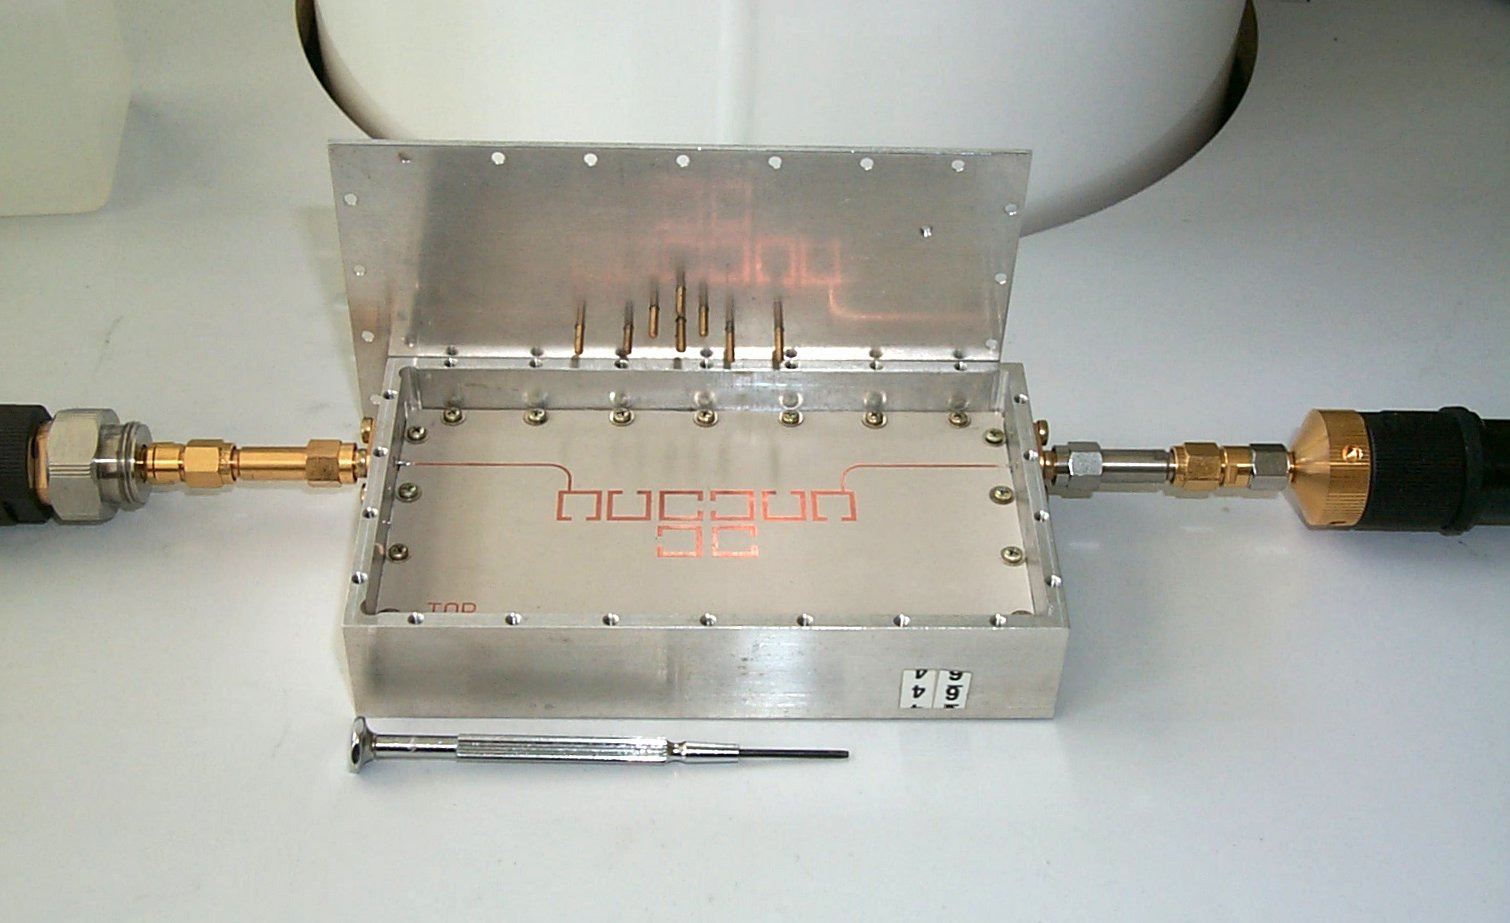
\includegraphics[scale=0.25]{fig/test-copper-open.jpg}
\vspace{-1em}
\caption{Copper test filter}
\label{figure:test-copper-open}
\end{figure}

\begin{figure}[ht]
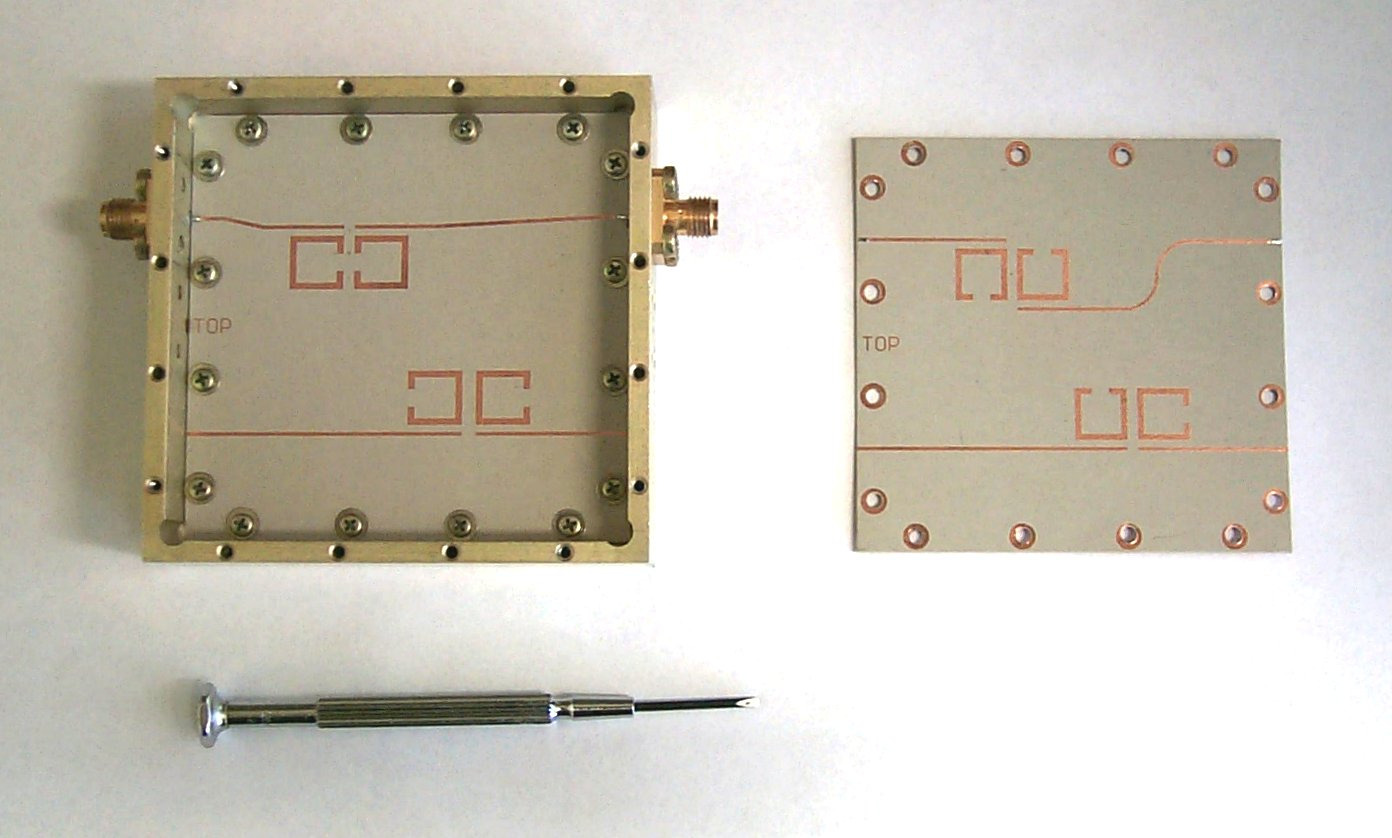
\includegraphics[scale=0.25]{fig/test-resonator-open.jpg}
\vspace{-1em}
\caption{Boards to test resonator coefficients}
\label{figure:test-resonator-open}
\end{figure}


% ------------------------------------------------------------------
\subsection{Testing}
Once tuned, the filter was measured to have the response shown in Figure 14. The lid appeared to reduce the stray couplings between non-adjacent resonators and improve the filter response. This effect was also observed when the HTS filter was tested.

\begin{figure}[ht]
\hspace{-4em}
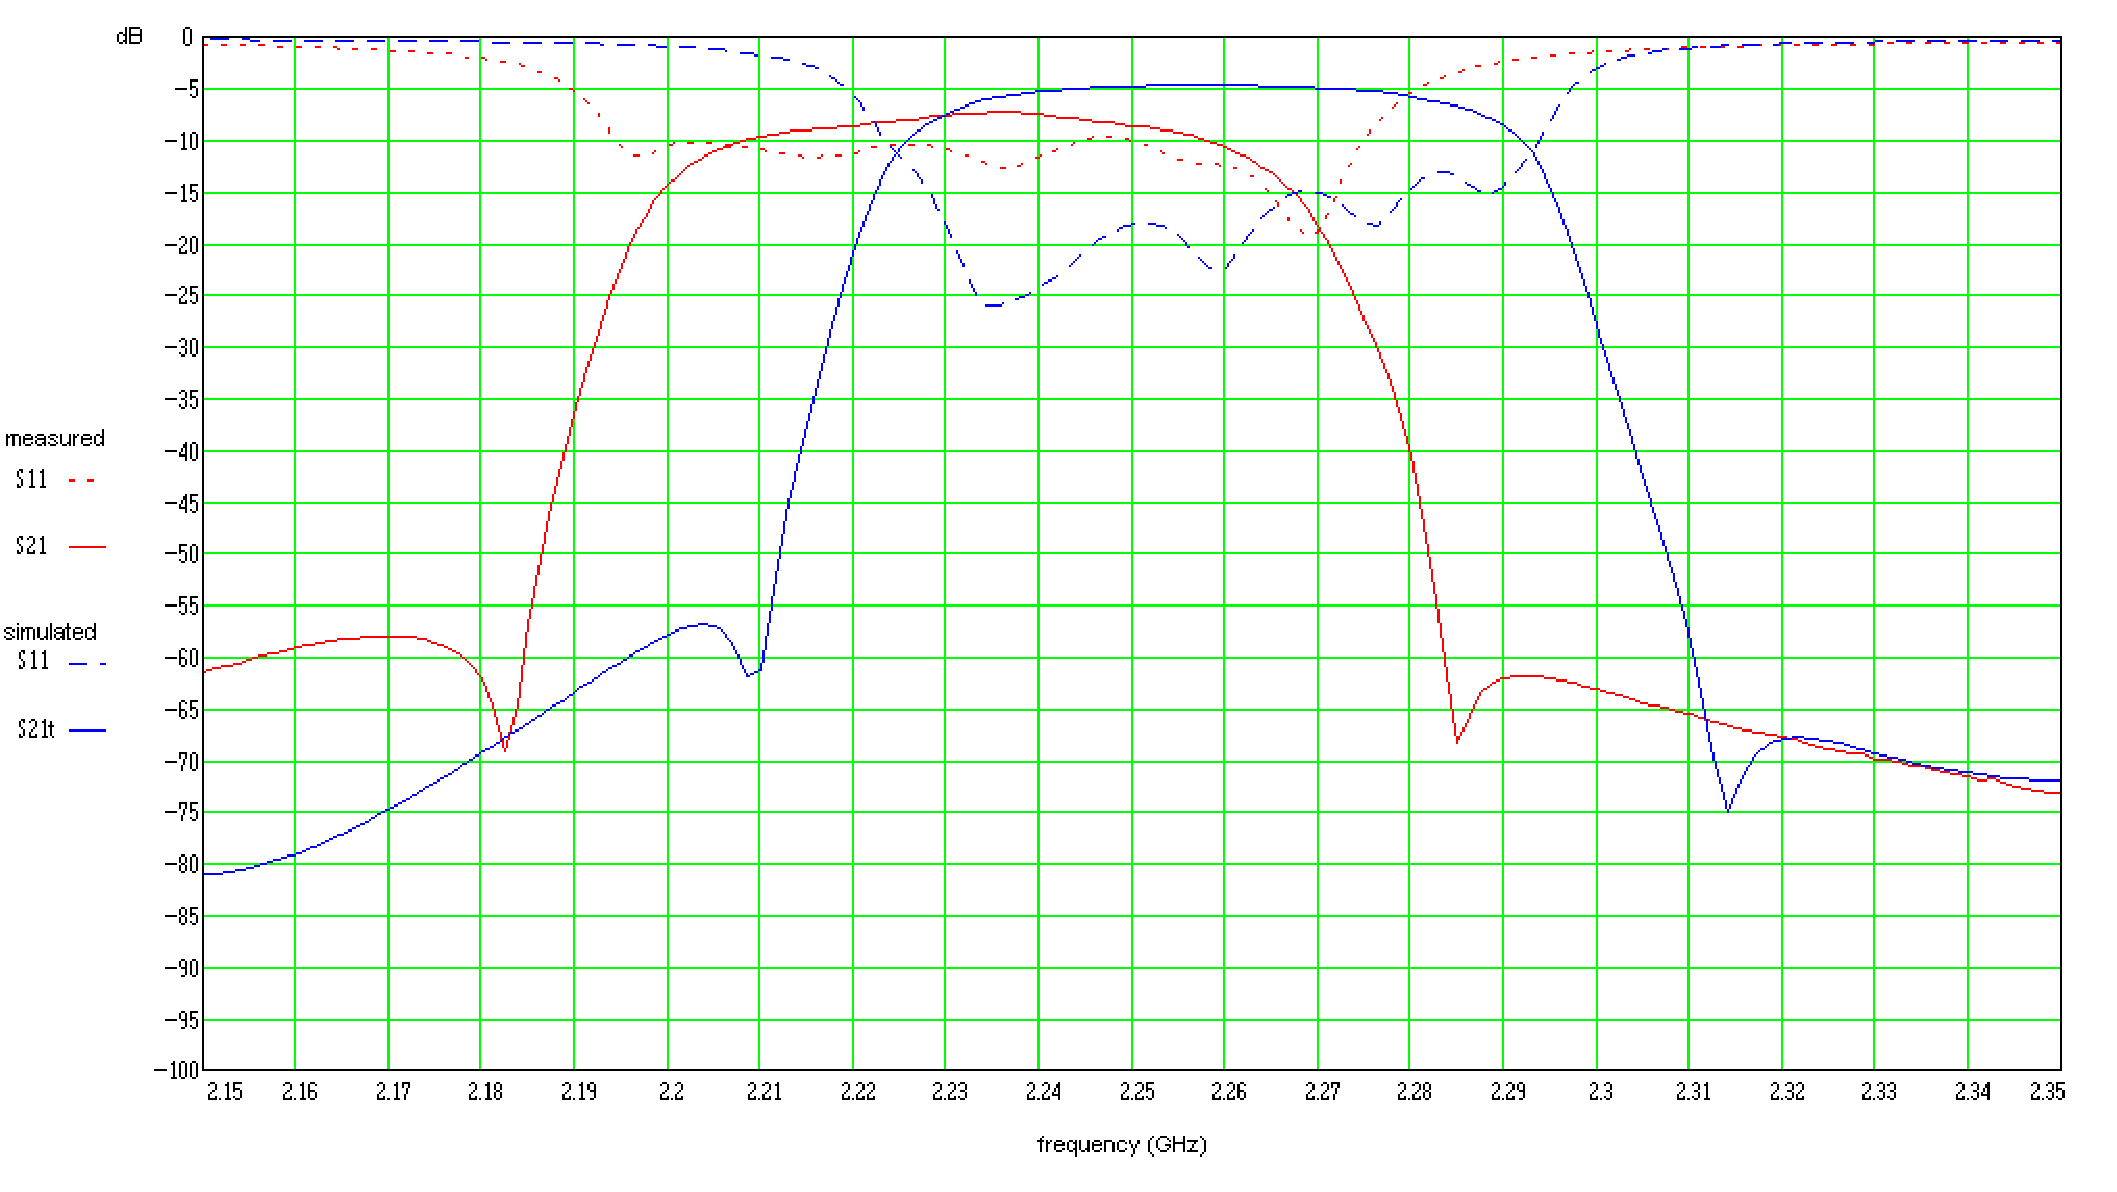
\includegraphics[scale=0.4]{fig/test-copper-response.pdf}
\vspace{-1em}
\caption{Response of copper test filter}
\label{figure:test-copper-response}
\end{figure}

\begin{figure}[ht]
\hspace{-4em}
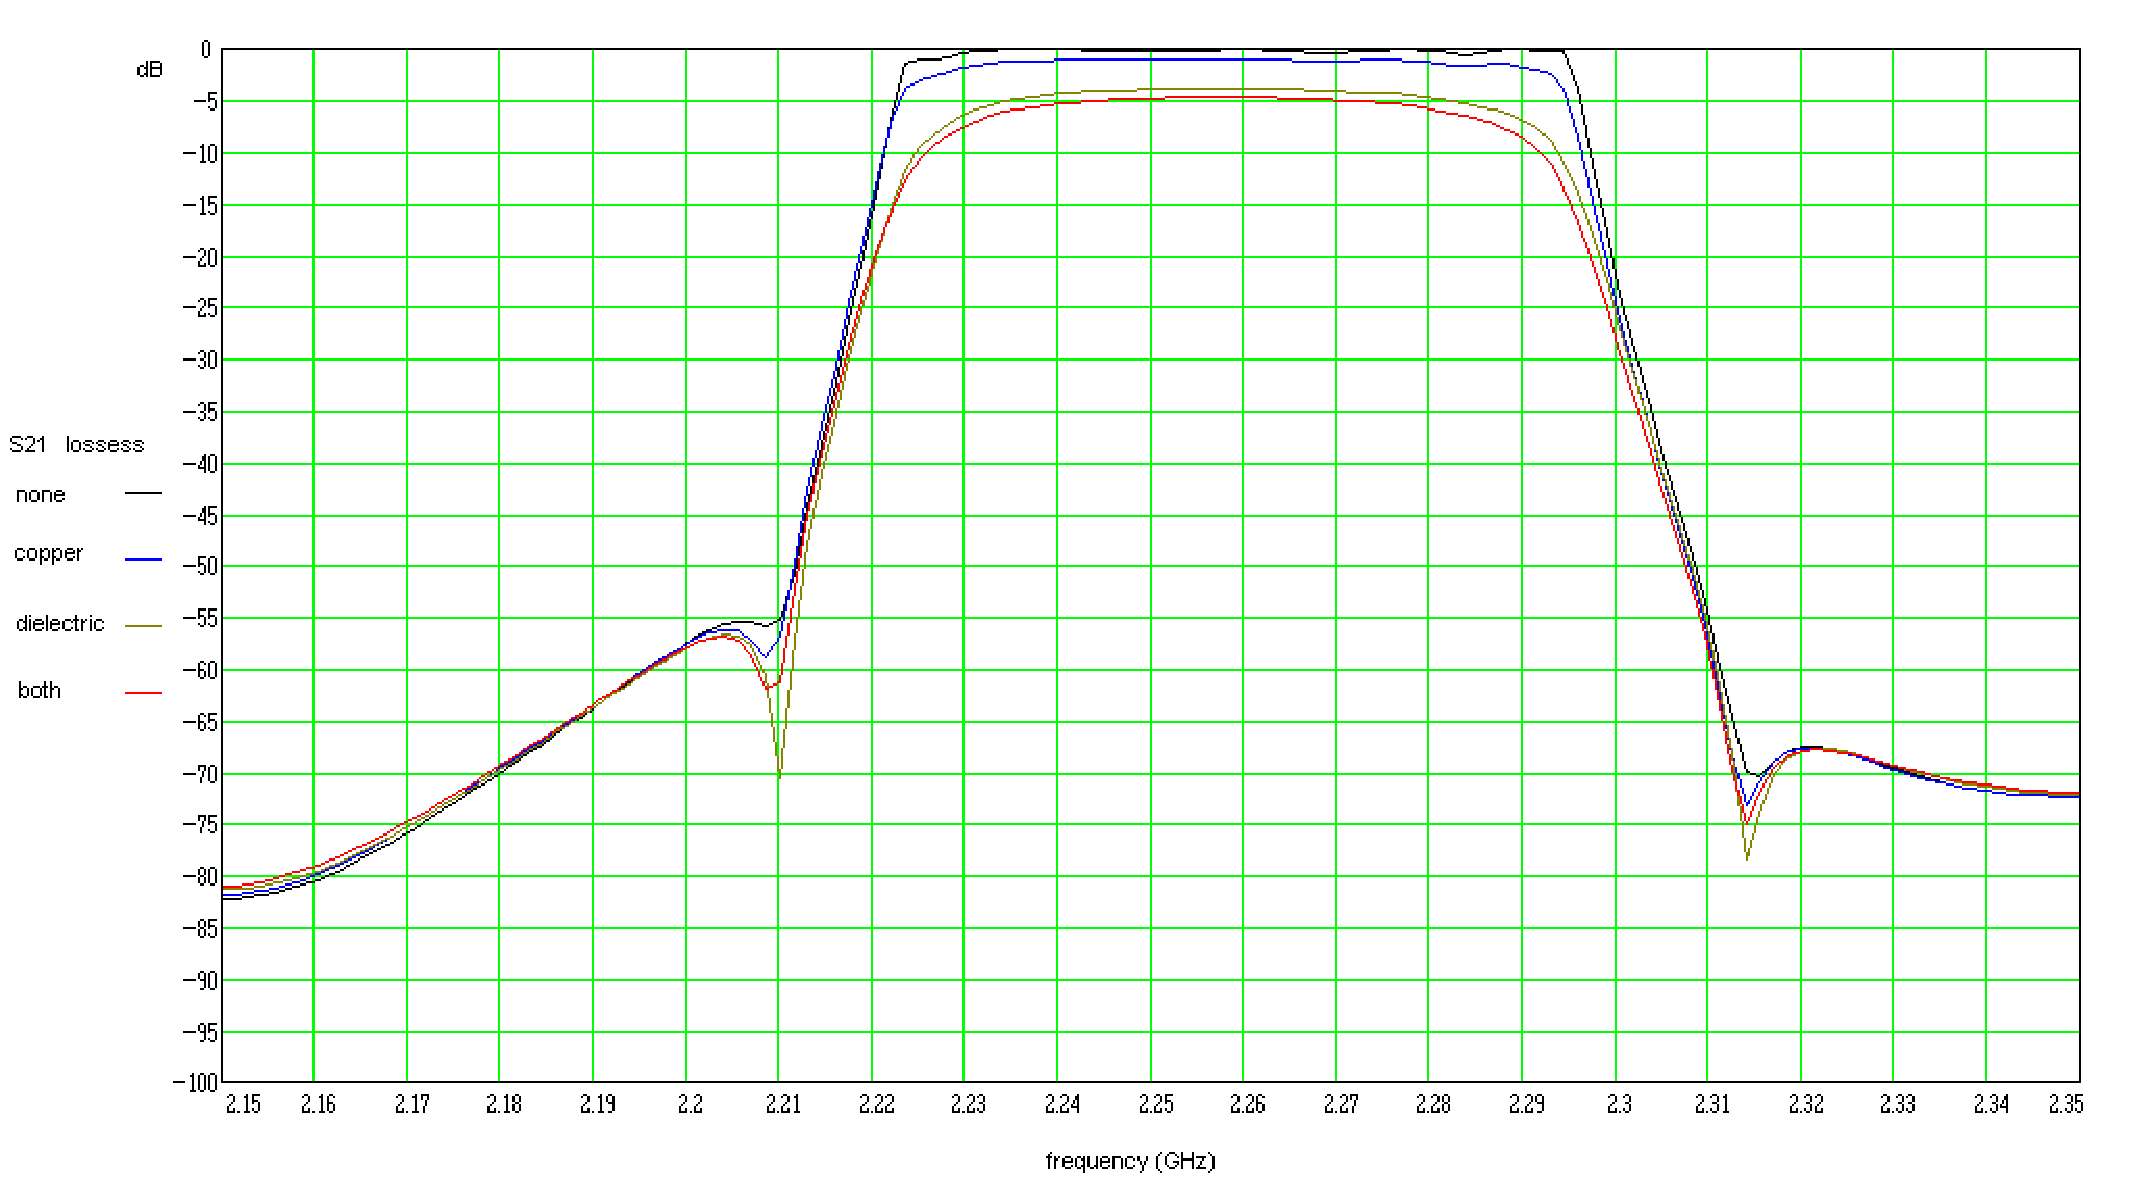
\includegraphics[scale=0.4]{fig/test-copper-loss.pdf}
\vspace{-1em}
\caption{Loss mechanisms}
\label{figure:test-copper-loss}
\end{figure}

The filter center frequency was about 25MHz too low and examination under the microscope revealed that it had been slightly over etched and had lost about 0.03mm all the way around. We simulated the filter with revised dimensions but it did not create the same effect. This leads us to believe that either the dielectric constant or height of the material is slightly different than what was specified. 

The rounding of the filter passband is due to copper and dielectric losses which we verified with the simulator (see figure 15). Examination of the diagram reveals that although there is a loss from the finite conductivity of copper, the large proportion is due to the loss tangent of the substrate (RT/Duroid 6010.5 loss tangent = 0.0023).

After seeing this we checked the loss tangent of the substrate material which we were planning to use for the HTS filter, Lanthanum Aluminate, LaAlO3. We was happy to discover that its loss tangent of 6.0E-5 compared with 2.3E-3 would present no problem.

With a filter of such a small fractional bandwidth (3 percent) we had expected to do a bit of tuning. Our next step was to obtain a lid and plant a forest of tuning screws which could be screwed down into the gap between the resonators. Each screw slightly decreased the fringe field in the gap and served to reduce the coupling between two resonators. This allowed us to slightly alter the stop band response. The lid with the screws can be seen in Figure 12.

To correct the center frequency of the filter we experimented with the possibility of trimming a few hundred microns off the end of the resonators with a razor knife. The characterisation boards came in useful for this purpose as their were 8 resonators which we could butcher and directly see the effect on frequency and coupling. 

With a steady hand it was possible to trim lengths of line equivalent to approximately 5MHz at a time off the ends of the resonators. The effect on the coupling coefficients depends on the types of coupling the resonator being modified is a part of. Electric coupling is most effected as the majority of the action takes place via electric fringe fields at the ends of the resonators. Conversely, magnetic coupling is least effected as the magnetic fringe fields circulates the lengths of the resonators away from the ends.

From simulation it was determined that even trimming of the lines does not significantly effect the shape of the filter response as it is shifted by a few tens of MHz. However, reproducibility between hand modifications is difficult to obtain. With more practice and frequent examinations under a measuring microscope it should be possible to trim down the resonators and center the filter on the correct frequency though this has not yet been attempted.

Apart from fabrication tolerances, this prototype was deemed a success and gave a degree of confidence to the HTS design.

%!TEX root = ../Main.tex

% ------------------------------------------------------------------
\section{Fabrication of HTS Filter}
The HTS design was similar to the copper design except for a higher dielectric constant, E=24 and a thinner substrate h=0.5mm. The higher dielectric constant reduces the line length required to resonate at the same frequency. It also decreases the width of the 50 Ohm lines. The whole filter becomes much smaller and compact. The final design is shown in Figure~\ref{figure:design-hts-layout}.

\begin{figure}[ht]
\begin{center}
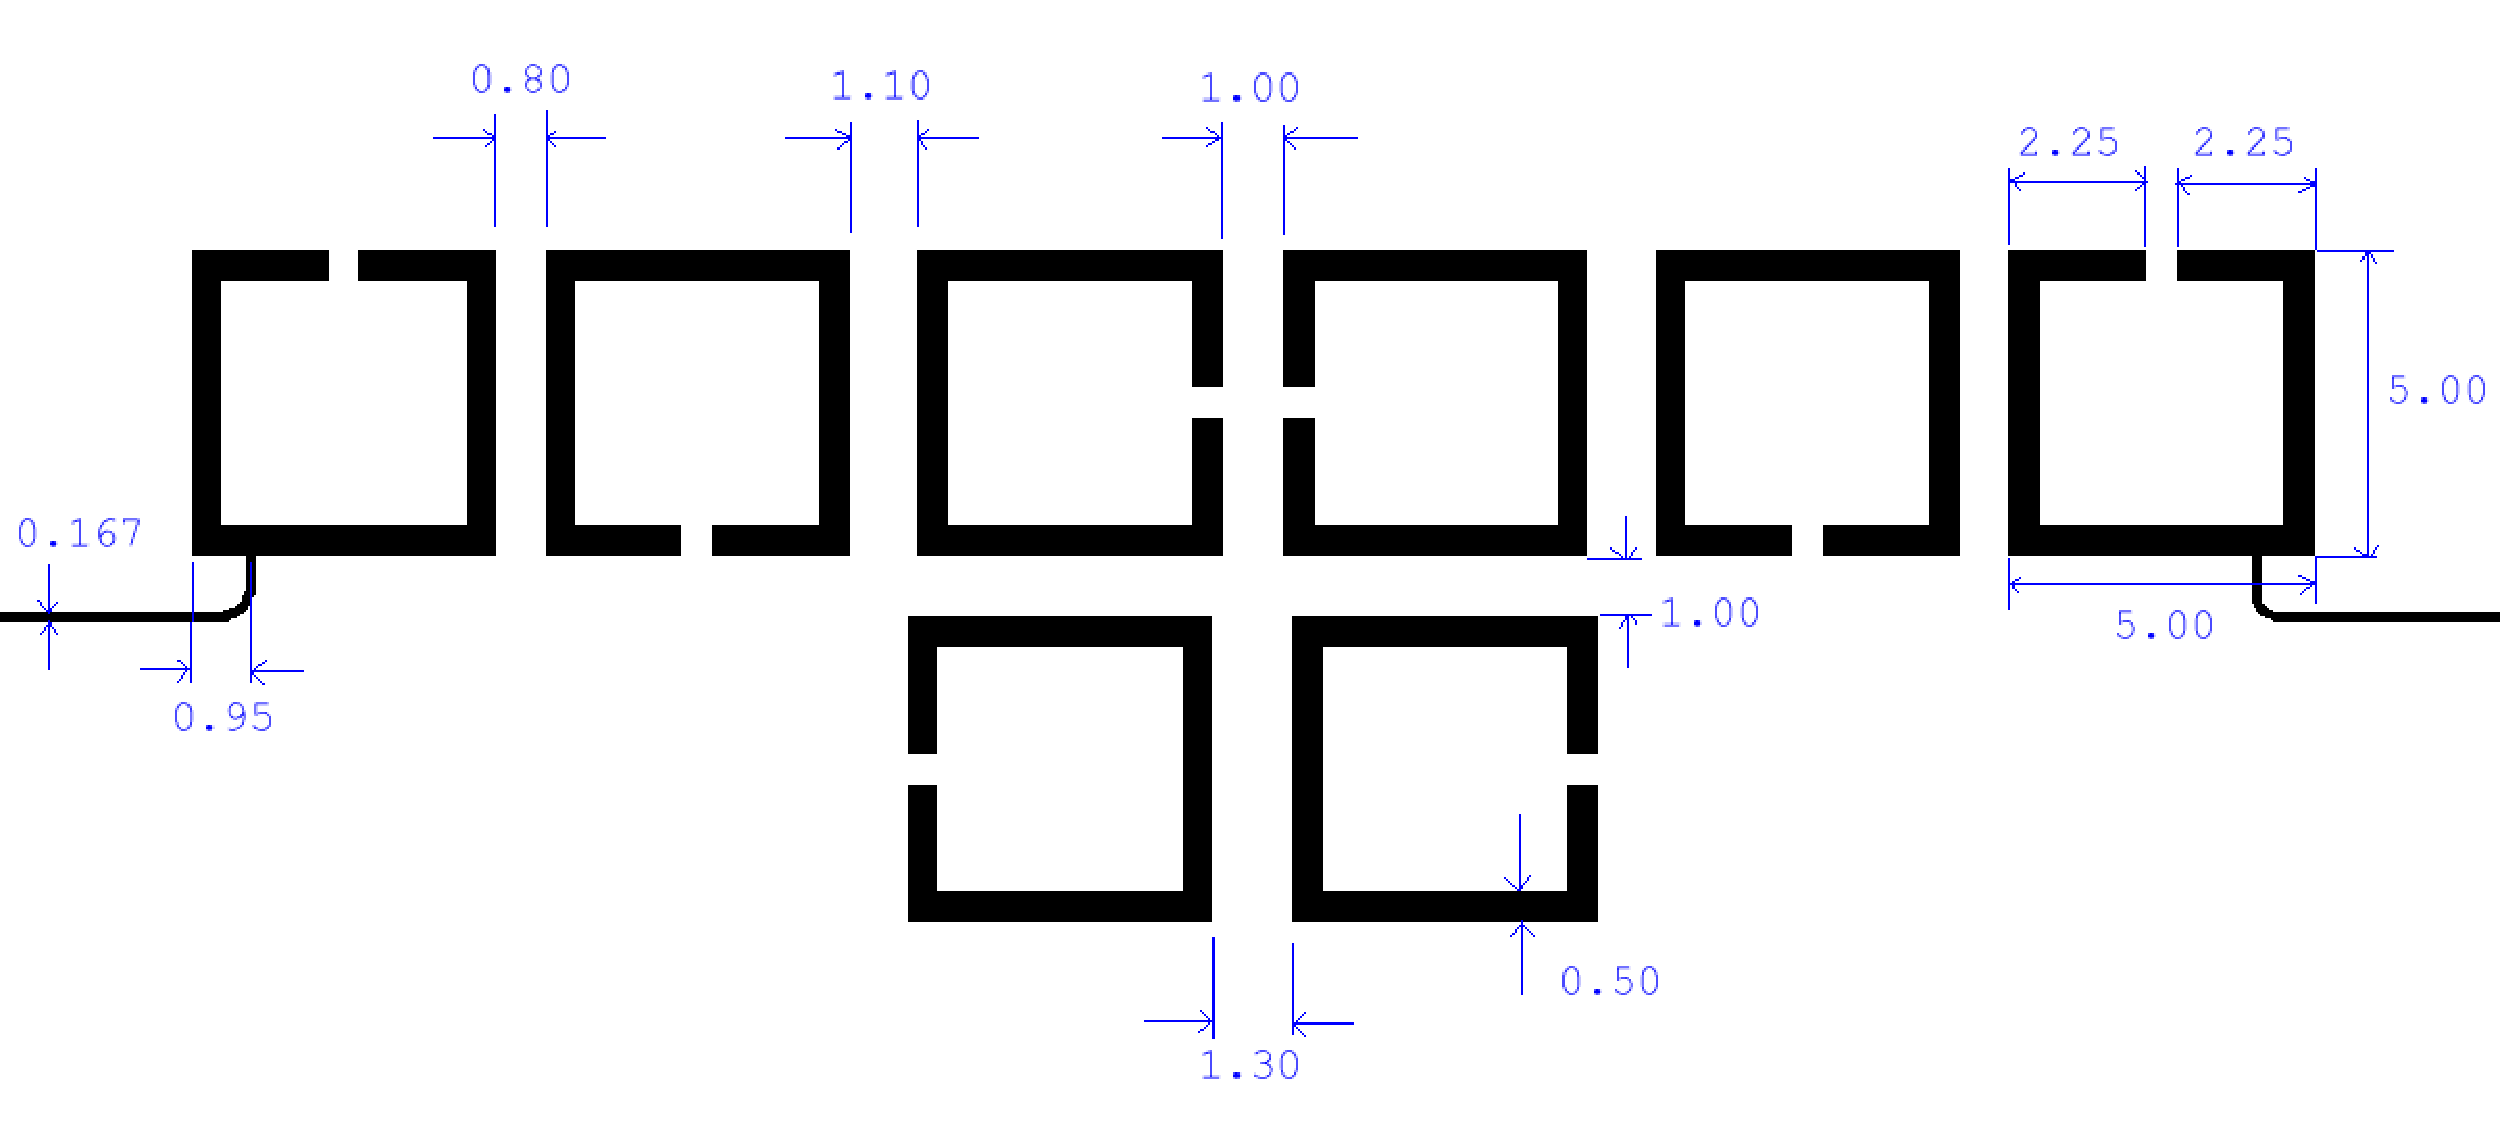
\includegraphics[scale=0.3]{fig/design-hts-layout.pdf}
\end{center}
\vspace{-1em}
\caption{HTS filter layout (dimensions in mm)}
\label{figure:design-hts-layout}
\end{figure}


% -----------------------------------------------------------------------------
\subsection{Fabrication}
The HTS material used was double sided YBCO thin film on a Lanthanum Aluminate substrate. Both sides were flashed with gold to provide a surface which could be soldered to. The HTS material is quite expensive so an effort was made to fit the filter on one half of a 50mm diameter wafer.

The filter was fabricated at the Linfield HTS lab and mounted in an existing box. The box was made from a Silicon Carbon Aluminate (SiCAl) base with copper sidewalls and a brass lid. The SiCAl base provides a good thermal expansion match with the LaAlO3 substrate and is also highly conductive. Silver paste was used to provide a good thermal and electrical contact between the ground plane and the base.

The SMA connectors used had a sliding center pin to account for the thermal contraction of the material. Indalloy 290 solder (In 97\% Ag 3\%) was used to attach the connector pins to the feed lines.

A picture of the final HTS filter is shown in Figure~\ref{figure:test-hts-open}. The picture shows a mess on the left hand feed line of the HTS filter. When the filter was first cooled this track was pulled from the substrate. Although the connector pins where supposed to slide with the contraction of the device, this did not happen. One possibility is that the pins were sticking in their housing as there was not enough mechanical strength in the YBCO-LaAlO3 bond to prevent it from breaking. Future designs will have the end of the feed several line widths wide to provide a stronger bonding surface.

\begin{figure}[ht]
\begin{center}
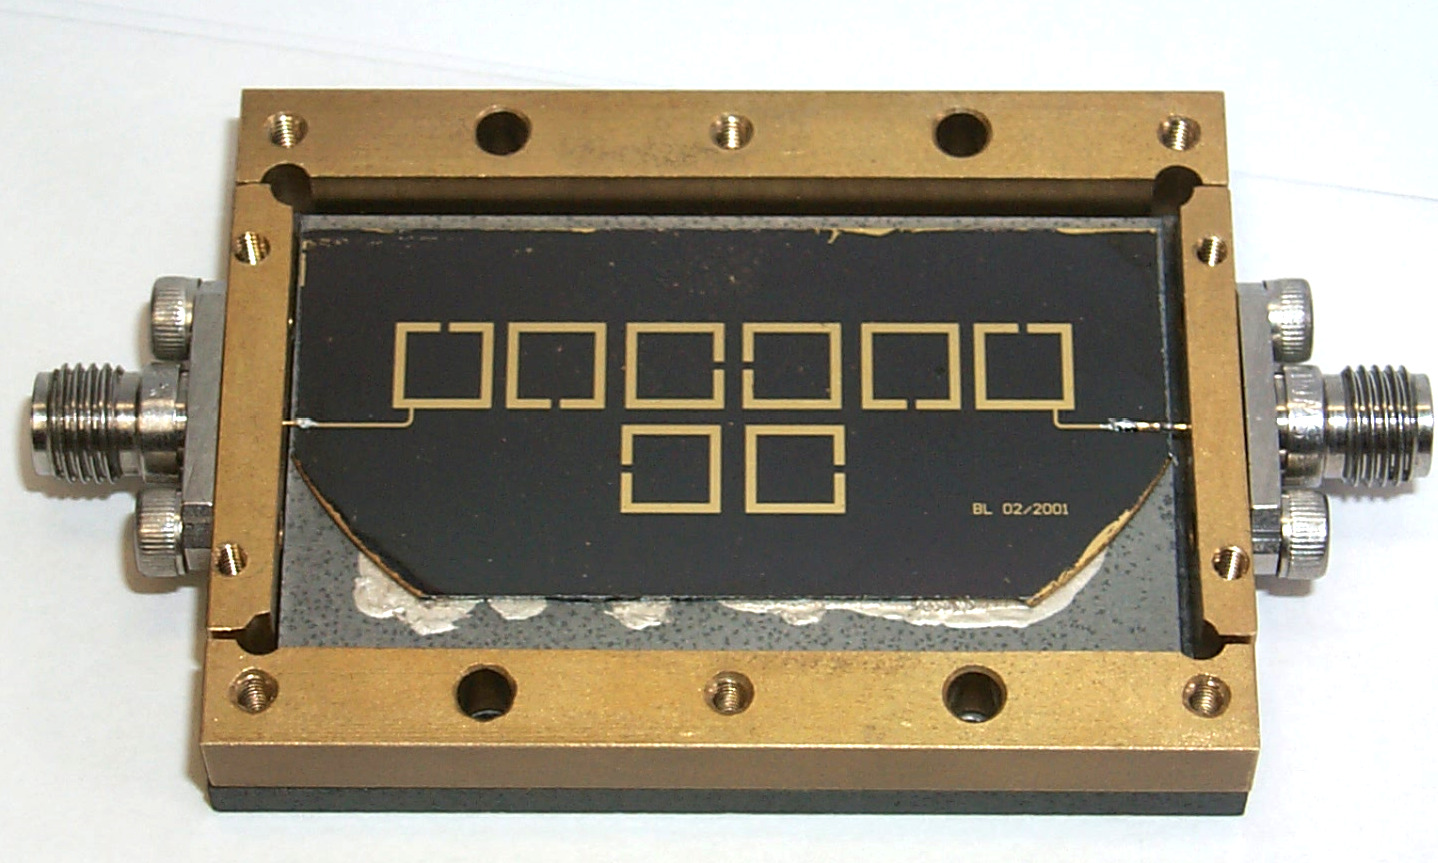
\includegraphics[scale=0.25]{fig/test-hts-open.jpg}
\end{center}
\vspace{-1em}
\caption{HTS Filter}
\label{figure:test-hts-open}
\end{figure}

\begin{figure}[ht]
\begin{center}
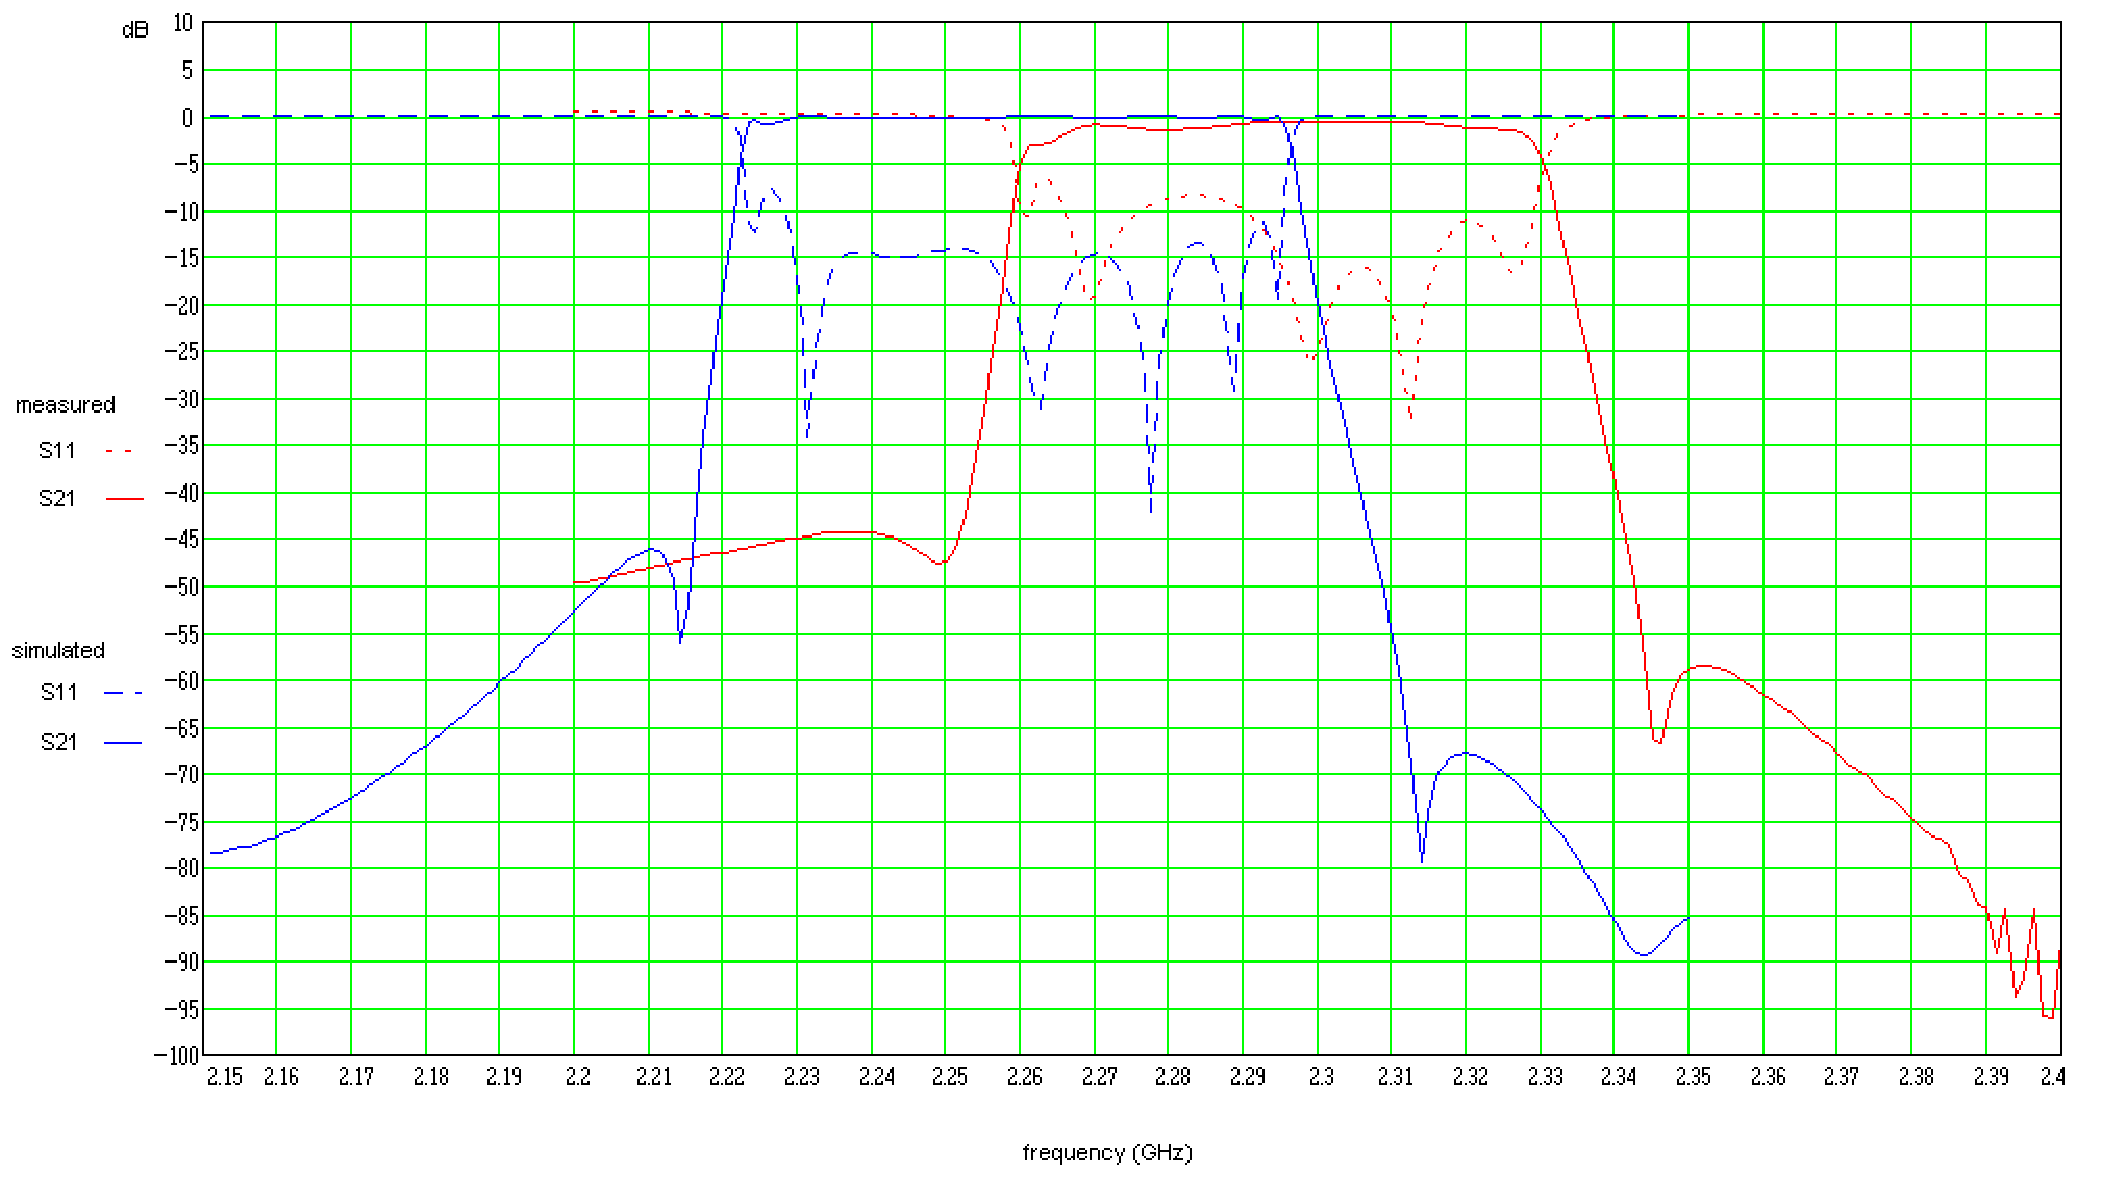
\includegraphics[scale=0.4]{fig/test-hts-response.pdf}
\end{center}
\vspace{-1em}
\caption{HTS filter response}
\label{figure:test-hts-response}
\end{figure}


% -----------------------------------------------------------------------------
\subsection{Result}
Once cooled, the filter gave the response shown in Figure~\ref{figure:test-hts-response}. The shape of the response was acceptable, withoug the rounding of the passband seen in the copper. The insertion loss in the center of the band was measured at 0.7dB.

There is a slight nick in the lower side of the passband of the simulated response, who's effects are also seen in the measured response. As mentioned earlier, although the separations of the resonators can be adjusted to give the coupling coefficient required by the filter synthesis tables, the filter synthesis tables to not account for non-adjacent couplings. This has caused the nick in the passband and also the asymmetry in the stop band. There will always be a degree of tuning required if perfect symmetry is desired.

This time, the filter response was 35MHz too high. A HTS film behaves slightly differently to how a perfectly conducting metal would~\cite{Shen:hts}. The simulator used does not take these effects into account though simulators are available which do. There is also a degree of uncertainty in the cooled dielectric constant of the material, it is often quoted as \emph{approximately} 24. 


% ------------------------------------------------------------------
\subsection{Tuning}
As with the copper filter the next step was to plant tuning screws in the box lid and attempt to clean up the response. Screws were placed into the fringe fields between the resonators and at the resonator ends to adjust the center frequency.

There was a difficulty in adjusting the tuning screws when the filter was in the sealed vacuum dewar. The first attempted solution to this problem was to screw a test device onto a copper block. The base of the block was then immersed in liquid nitrogen leaving the filter above the surface. This provided a moderate cooling rate for the filter as well as easy access to the screws. Unfortunately moisture had condensed from the atmosphere and froze onto both the filter body and the part of the block which was above the nitrogen.

As the YBCO HTS film is susceptible to moisture, this procedure was deemed unusable as the device would be ruined when it was re-warmed and the ice liquefied. It is important to note that the filter box is not sealed as there are gaps in the body to account for the thermal contraction of the copper walls.

The next solution was to drill a set of holes in a perspex dewar lid and insert rubber bungs with screwdrivers set through the middle. A picture of the setup used is shown in Figure~\ref{figure:test-hts-fridge}.

As the bung cannot be tilted too far for risk of breaking the vacuum seal, there were two separate screwdrivers installed so all screws could be reached.

Even with vacuum grease sealing the rubber-perspex and rubber-screwdriver interfaces there is a small amount of air leakage though it is not problematic. The white circle in the center of the cold plate consists of nitrogen and water vapor which has leaked into the dewar and frozen.

Although the tuning setup was successful, the range of tuning possible was inadequate to improve the filter response. The zero on the low side of the response could be deepened slightly and the passband ripples smoothed out a little. The number of tuning variables ( number of screws) is large enough to make the tuning process  time consuming and more a process of trial and error than anything else.

More importantly, the center frequency of the resonators was found to be tunable by less than 5MHz or so, which was insufficient to correct the 35MHz difference in center frequency.

\begin{figure}[ht]
\begin{center}
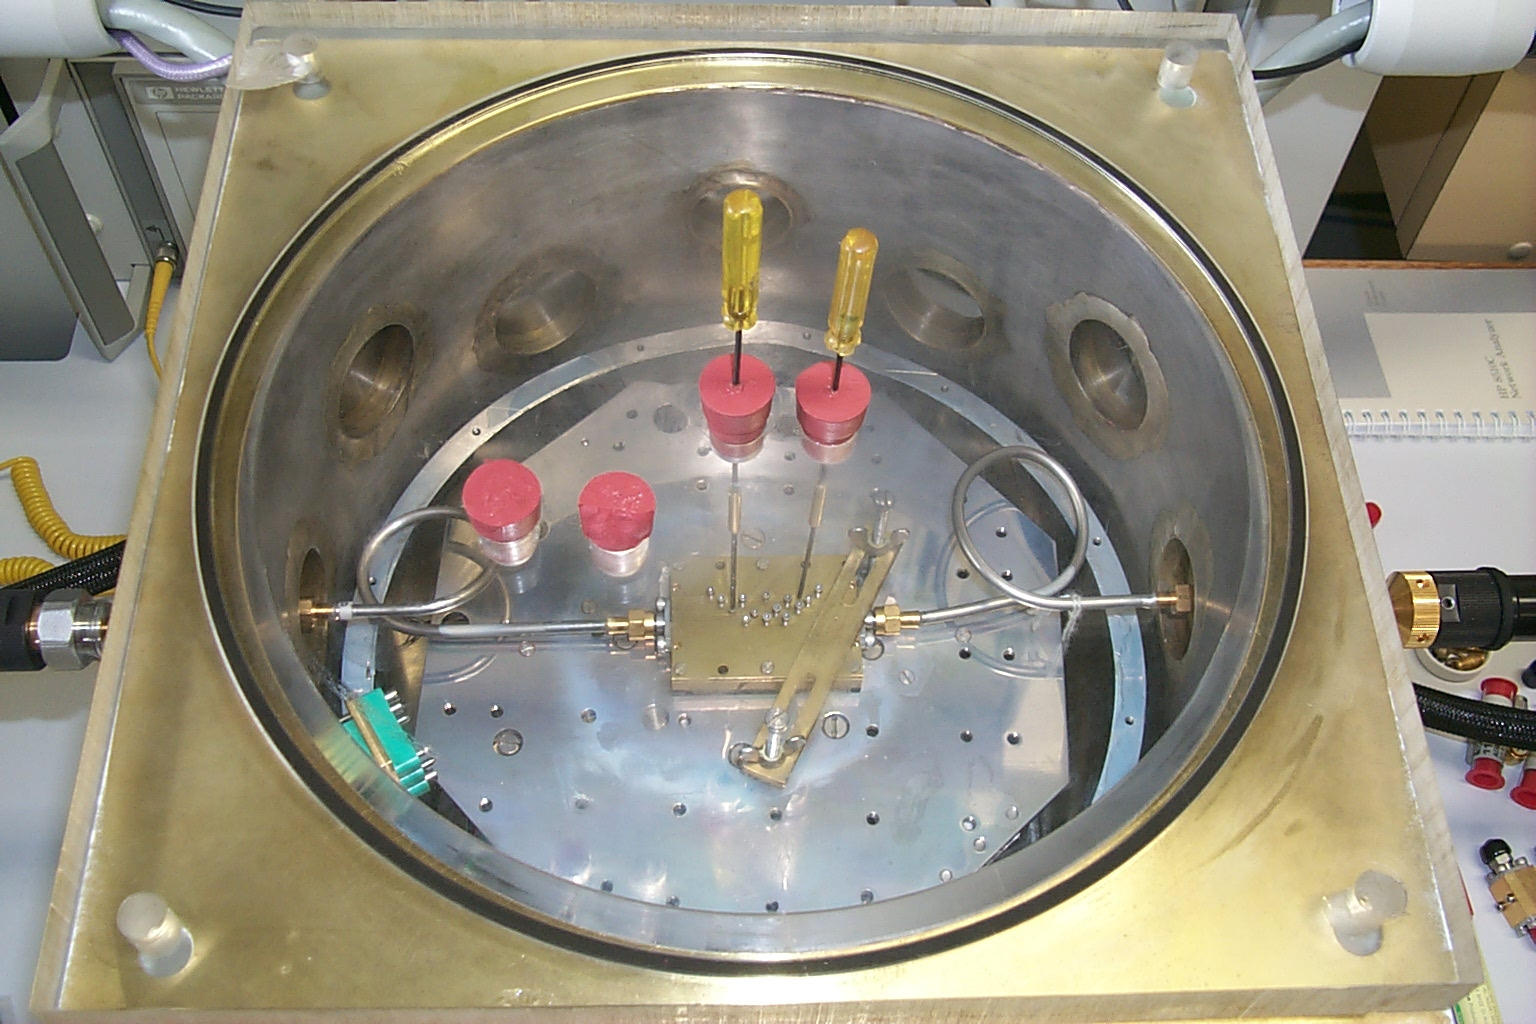
\includegraphics[scale=0.2]{fig/test-hts-fridge.jpg}
\end{center}
\vspace{-1em}
\caption{HTS filter in fridge}
\label{figure:test-hts-fridge}
\end{figure}


%!TEX root = ../Main.tex
\section{Conclusion and Future Work}

Future work would be to repeat the filter sign process, but using a center frequency intentionally 35MHz too low, and have it fabricated on the other half of the wafer used for the first filter. The properties of the substrate should remain relatively constant over the entire wafer and if all goes to plan, the new filter would come out right on frequency.

This trick may or may not work if another wafer is used. There are a number of things to consider, one of them being whether the frequency shift really was due to inaccuracies in the dielectric constant, the simulation model being used, or a combination of both. There is also the question of how other properties of the material vary between wafers.

A more promising and reproducible avenue is to design a filter grossly too low, say 50MHz and have it trimmed down until it is at the right frequency. The Marsfield CTIP site has a focused ion beam machine which should be capable of trimming filters to the correct lengths. From simulation, it was found that the center frequency of the filter can be shifted by this amount without adversely effecting the overall filter response. 




\medskip
\textbf{Acknowledgments}
Work performed as a summer scholar at the Australia Telescope National Facility (ATNF) receivers group. Thanks to Russell Gough and Graham Gay for help and advice, and for building the HTS tuning setup. Thanks to Jia Du and others at the Linfield HTS Lab for fabricating the HTS filter.

\clearpage{}
\bibliographystyle{plain}
\bibliography{Main}

\end{document}
